\chapter{Redes neuronales artificiales evolutivas mono-objetivo}\label{evoMonoObjetivo}
% \begin{quotation}
% \begin{small}
% 		\textit{El pesimista es un optimista con experiencia.}\\
% 		\textit{El pesimista es una persona previsora y bien informada.}
% \end{small}
% \begin{flushright}
% François Truffaut.\\
% Anónimo.
% \end{flushright}
% \end{quotation}
\section{Motivación}
\noindent En este capítulo hablamos fundamentalmente del diseño de ANNs híbridas mediante
AEs, usando un
algoritmo al que hemos llamado CBFEP (\textit{Combined Basis Function Evolutionary
Programing})
\cite{Gutierrez2009,Gutierrez2007}. Este algoritmo fue diseñado como paso previo al diseño
de ANNs mediante algoritmos evolutivos multi-objetivo, (\textit{Multi-Objective
Evolutionary Algorithms}, MOEAS) \cite{Deb2004,Coello2007}, ya que en un futuro pensamos
incorporar ANNs híbridas junto con MOEAs para el diseño de modelos de red para
multi-clasificación de
patrones.

A continuación se muestra una breve introducción sobre el entrenamiento de ANNs con AEs y
sobre
las metodologías existentes, para posteriormente dar paso al algoritmo CBFEP.

\section{Entrenamiento de redes neuronales evolutivas}\label{enganio}
\noindent La Computación Evolutiva (\textit{Evolutionary Computation},
EC) \cite{Holland1992}, es una rama de la ciencia que interpreta la naturaleza como una
inmensa máquina de resolver problemas, y trata de encontrar el origen de dicha
potencialidad para reutilizarla en sus propias aproximaciones.
% El concepto de EA describe un conjunto de sistemas para resolver problemas mediante el
% ordenador, que usan un modelo computacional similar a los procesos evolutivos existentes
% en la naturaleza. Es decir, un modelo basado en el principio darwiniano de reproducción
% y
% supervivencia de los individuos que mejor se adaptan al entorno en que viven.

La utilización de métodos de naturaleza heurística para el entrenamiento de ANNs
surge en la década de los 90 (ver sección \ref{redesheuristicas} del capítulo
\ref{redesneuronales}). Las motivos principales que sugieren el uso de este tipo de
técnicas vienen determinados, en gran medida, por las limitaciones presentadas y
comentadas anteriormente por los algoritmos clásicos de aprendizaje (ver sección
\ref{mClasicos} del capítulo \ref{redesneuronales}). Dentro de los métodos
heurísticos, los EAs son los más utilizados para el diseño de modelos de red, ya
que presentan una metodología muy útil a la hora de optimizar la topología y los pesos de
una ANN, y existen muchas aplicaciones al respecto, tanto para clasificación de patrones
\cite{Bishop2006,Fu2004,Scheme2007,Paliwal2009} como para regresión
\cite{Valero2007,Hervas2007c,Hervas2007b,Hervas2009,Gutierrez2008,Gutierrez2009a,
Gutierrez2009b,Gutierrez2009d}. Los EAs \cite{Back1996,Back1997,Eiben2003} son eficientes
para encontrar un conjunto de pesos para las conexiones cercanas al óptimo, sin utilizar información
sobre el gradiente, y
la función de aptitud de los individuos no tiene porque ser diferenciable. Los EAs pueden
tratar espacios complejos, no diferenciables y multimodales. La evolución de las
arquitecturas de ANNs permite adaptar sus topologías a diferentes tareas sin la
intervención humana, y por lo tanto, proporciona una aproximación al diseño de las mismas
de manera automática, ya que tanto los pesos de conexión y como la arquitectura se pueden
evolucionar.

El entrenamiento de ANNs mediante EAs es un buen ejemplo para llevar a
cabo el dilema explotación/exploración en un algoritmo de búsqueda \cite{Lozano2008}.
Este método de aprendizaje puede resultar lento si se compara con otros métodos de
entrenamiento clásicos, sin embargo, los EAs son muchos menos sensibles a las condiciones
iniciales del entrenamiento, buscan una solución
global y óptima y no requieren el cálculo del gradiente. Si tenemos en cuenta
la dificultad que implica el establecimiento de una arquitectura adecuada junto con el
aprendizaje de los correspondientes pesos de la ANN, la utilización de EAs para el
diseño de la estructura y la optimización de los coeficientes de una ANN está
ampliamente justificada.

De la utilización de los EAs para la optimización de ANNs surgen las
denominadas Redes Neuronales Artificiales Evolutivas (\textit{Evolutionary
Artificial Neural Networks}, EANNs) \cite{Yao1999}. El lector puede consultar varios
trabajos y estados del arte sobre este aspecto
en \cite{Zhang2000,CantuPaz2005,Ludemir2006,Ou2007}.

Existen varias formas \cite{Yao1999} de abordar el entrenamiento de una
ANN con un EA, aunque son tres las más utilizadas:
\begin{description}
\item[Evolución de los pesos:] En este caso se fija la arquitectura de la red, número de
capas ocultas, número de nodos en capa oculta y número de conexiones, y se
desarrolla una búsqueda global en el espacio de los pesos (valores de las conexiones).
Esta técnica conlleva tener una gran experiencia por
parte de los diseñadores, y realizar procedimientos de prueba y error, partiendo de
diferentes topologías para un problema en cuestión. Además, es muy importante la elección
de los operadores genéticos de recombinación que se utilicen y la codificación de los
pesos que se haga (en la actualidad la codificación se hace mediante números reales).
\item[Evolución de la arquitectura:] Seleccionar la arquitectura
de una ANN es una difícil tarea, y las EANNs pueden encontrar
automáticamente una buena arquitectura que no produzca sobre-entrenamiento o falta de
aprendizaje en el conjunto de generalización. En este caso, se
suele partir de una inicialización aleatoria de los pesos y, tras la ejecución de un
EA, se suelen realizar varias iteraciones de un algoritmo BP clásico.
El diseño de una arquitectura óptima de una ANN se puede formular como un
problema de búsqueda en el espacio de arquitecturas, donde cada punto representa una
arquitectura diferente. Dados algunos criterios de rendimiento, como por ejemplo el error
más bajo de entrenamiento, la menor complejidad de red, etc, el nivel de rendimiento de
todas las arquitecturas forma una superficie discreta. El diseño de la
arquitectura óptima es equivalente a encontrar el punto más alto de esta superficie.
\item[Evolución de los pesos y la arquitectura simultáneamente:] Con esta \newline estrategia se
evolucionan simultáneamente los pesos y la arquitectura de la red. Cada individuo de la
población especifica tanto la arquitectura como los pesos de conexión. El operador
genético que se suele utilizar es la mutación, tanto paramétrica (modificación de los
pesos de la ANN) como estructural (modificación de la topología). El cruce en
ocasiones puede que no proporcione buenos resultados, ya que recombinar una parte de una
ANN con otra parte de otra, posiblemente hará que ambas redes pierdan
funcionalidad \cite{Angeline1994}. Por otra parte, existe el problema de la permutación o
del engaño \cite{Yao1999}, que consiste en que dos redes que ordenan
sus nodos ocultos en forma diferente tienen distinta representación, pero pueden ser
funcionalmente equivalentes, con lo que la probabilidad de producir una mejor descendencia
por recombinación a partir de ellas es baja. Por ejemplo, las ANNs mostradas
por las figuras \ref{enganio1a} y \ref{enganio2a} son equivalentes, pero tienen distintas
representaciones del genotipo, como se ve en las figuras \ref{enganio1b} y
\ref{enganio2b}, usando el esquema de codificación directo. En general, cualquier
permutación de los nodos ocultos producirá ANNs funcionalmente equivalentes,
pero con distintas representaciones del genotipo. A pesar de ello hay autores que no
consideran este problema demasiado importante y sugieren que cambiando los tamaños de
población y la selección de individuos se reduce considerablemente.

\begin{figure*}[htb]
\centering
\subfloat[]{\label{enganio1a}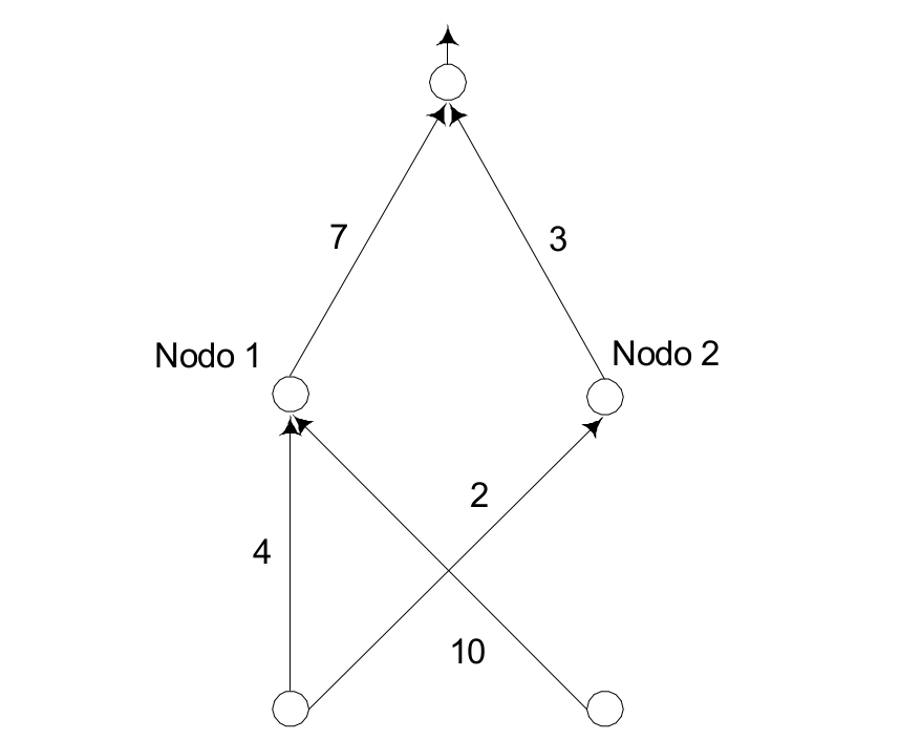
\includegraphics[width=.35
\textwidth]{figuras/enganio_1a.jpg}}
\subfloat[]{\label{enganio1b}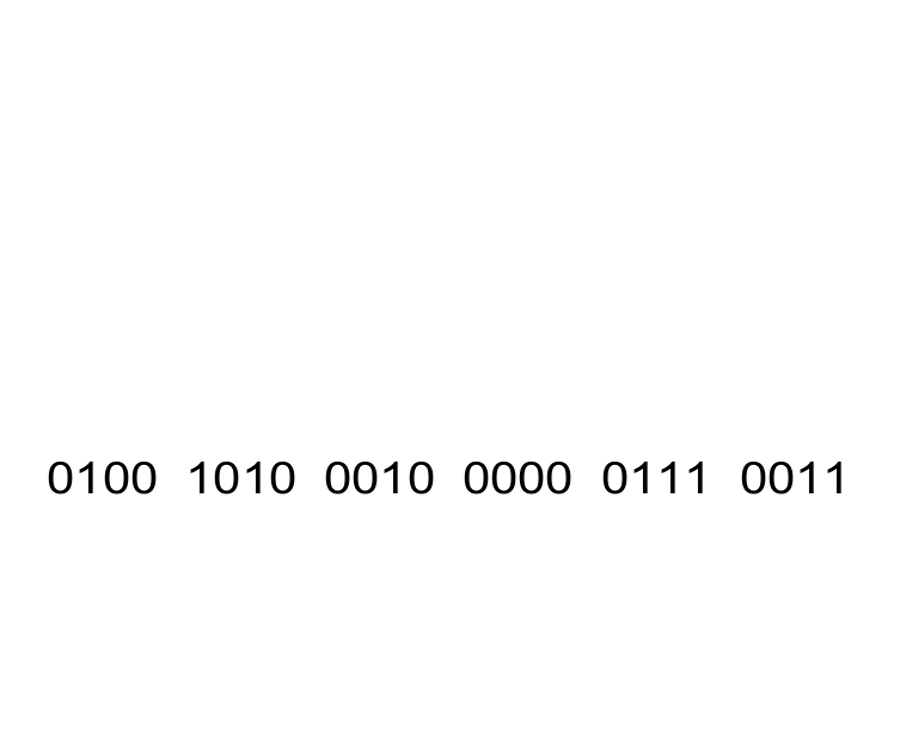
\includegraphics[width=.35
\textwidth]{figuras/enganio_1b.jpg}} \\
\subfloat[]{\label{enganio2a}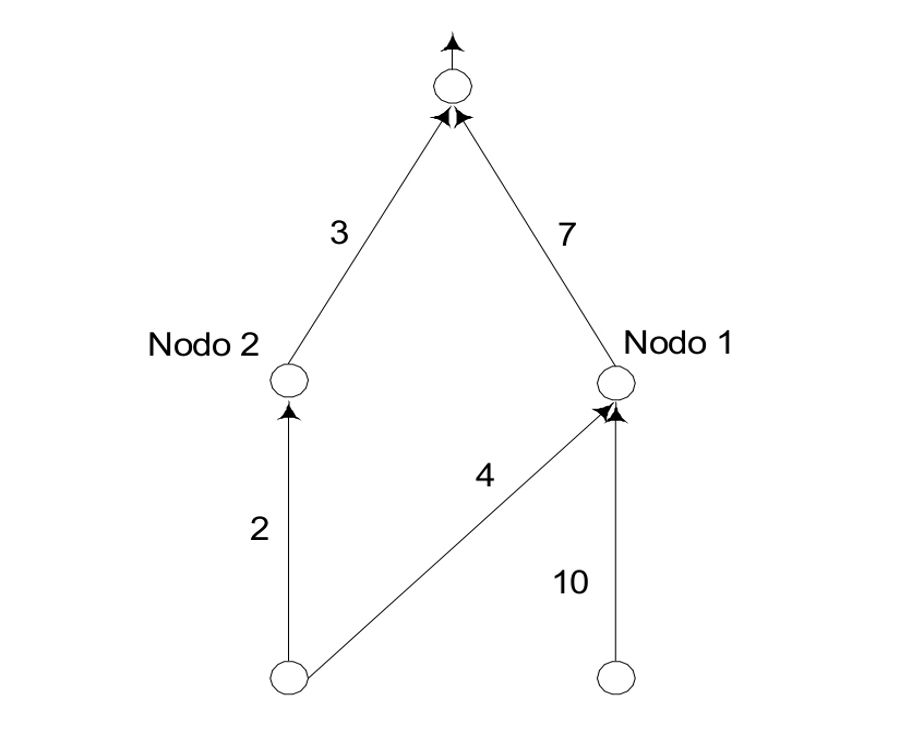
\includegraphics[width=.35
\textwidth]{figuras/enganio_2a.jpg}}
\subfloat[]{\label{enganio2b}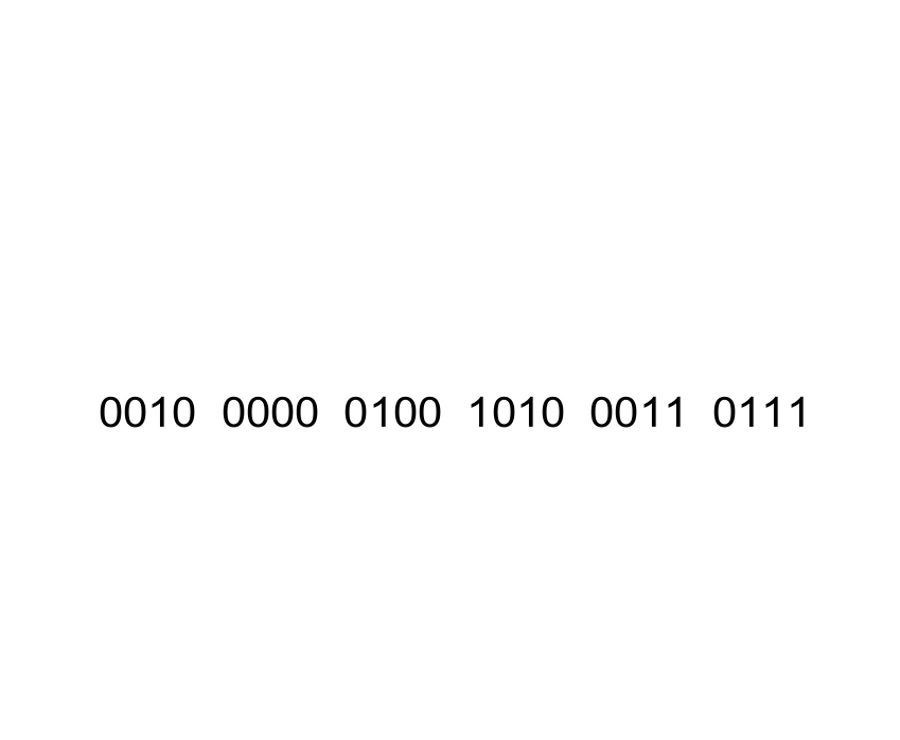
\includegraphics[width=.35
\textwidth]{figuras/enganio_2b.jpg}}
\caption{Problema de la permutación. En a) y c) se muestran dos redes
equivalentes y en b) y d) sus representaciones genotípicas.}
\label{enganio}
\end{figure*}
% \item[Evolución de las reglas de aprendizaje:] Otro tipo de evolución en
% \textit{ANNs} (aunque menos usada) es la evolución de las reglas de aprendizaje junto
%con
% los pesos de la red \cite{Baxter1992}.
% Este tipo de evolución tiene que realizarse en entornos dinámicos pero estableciendo una
% serie de restricciones, como por ejemplo la forma básica de la regla de aprendizaje,
%para
% así reducir la complejidad de la representación, y una serie de asunciones: la
% actualización de los pesos depende solo de información local, y la regla de
% aprendizaje es la misma para todas las conexiones en una ANN.
\end{description}

\section{Codificación de redes neuronales evolutivas}\label{codificacion}
\noindent Es importante comentar que la codificación que se haga de la ANN
influye en el proceso del diseño de la misma. Hay dos tipos de codificación (ver con más
detalle en \cite{Yao1999}) :
\begin{description}
\item[Directa:] La arquitectura de la red se codifica directamente sobre un cromosoma,
describiéndola en todos sus aspectos, incluyendo los pesos de la misma. Este diseño  se
puede  realizar  conjuntamente  con  la  estimación  o  aprendizaje  de  los pesos,  o
hacerlo independientemente, usando un cromosoma para los pesos y otro para la
arquitectura. Este tipo de codificación permite definir con facilidad operadores de cruce
y de mutación, sin embargo, el problema de la codificación directa es que en el caso de
que las estructuras sean grandes crece su representación, lo que produce un algoritmo poco
eficiente. No obstante, existen posibilidades de reducir el tamaño de las matrices de
representación, si tenemos en cuenta algunas  de  las restricciones propias  de la  red
neuronal, como puede  ser que  no existan  conexiones entre los nodos de entrada.
\item[Indirecta:] Una codificación indirecta describe solamente la manera de
``ensamblar'' una ANN. El objetivo es minimizar la longitud del cromosoma que
representa a la estructura de la red, representando  algunas  características importantes
que la identifiquen. Un tipo de representación indirecta puede ser la representación
paramétrica, donde una red se puede representar como un conjunto de parámetros: número de
capas ocultas, número de nodos en cada capa y número de conexiones entre capas. Otro tipo
de representación indirecta puede ser mediante gramáticas, compuestas por reglas de
producción para construir arquitecturas. La codificación indirecta puede producir una
representación genotípica más compacta de la arquitectura de una red, pero quizás no sea
tan buena en la búsqueda de una red compacta con una buena capacidad de generalización.
\end{description}

En este trabajo de tesis el tipo de codificación que se utiliza es directa, pero no se
trabaja directamente con los pesos y/o estructura de la red, sino con una representación
orientada a objetos. Digamos, por tanto, que se trabaja a caballo entre el genotipo y el
fenotipo (interpretación del genotipo), ya que a cada una de las características de la
red se accede por medio de una clase \cite{Poo2007}. Cada conexión se especifica por un
valor binario, indicando si existe o no, y por separado se indica con un valor real el
peso de la misma. Como se verá más adelante no se considerarán operadores de cruce en la
evolución de los individuos de la población, con lo que no se asume un orden fijo entre
los distintos nodos ocultos. A nivel de programación e ingeniería del software, de manera
breve, cada ANN
queda representada
por: clases para representar las diferentes capas de la red (entrada, oculta,
salida) y el tipo de capa oculta, según esté formada por unidades puras o una hibridación
de estas; clases para representar el tipo de unidad de base, nodo o neurona
utilizados en cada capa (sigmoides, producto, base radial), y si es una neurona de entrada
o una neurona enlazada; y clases para representar enlaces entre dos nodos o neuronas y
su valor o peso.

En la siguiente sección exponemos un EA para el entrenamiento de ANNs híbridas como paso
previo a corto plazo de la incorporación de este tipo de ANNs a MOEAs.

\section{El algoritmo CBFEP}
\noindent Una vez comentadas las características básicas de un EA y las diferentes
metodologías usadas en la literatura para el entrenamiento de ANNs mediante EAs, pasamos
a describir un algoritmo que hemos diseñado para la obtención de modelos de red híbridos (ver
sección \ref{redesHibridas} del capítulo \ref{redesneuronales}) para clasificación de
patrones, teniendo en cuenta solo una función objetivo o función de aptitud. Hemos llamado
a este algoritmo CBFEP (\textit{Combined Basis Function Evolutionary Programing})
\cite{Gutierrez2007,Gutierrez2009}.

CBFEP es un EA que estima los parámetros y la estructura de la red de manera simultanea, lo que se
conoce como método TWEANN (\textit{Topology and Weight Evolving Artificial Neural
Networks}). La población de individuos está sujeta a operaciones de
replicación y de mutación, no usando operador de cruce debido a las desventajas
potenciales que ha demostrado tener en la evolución de ANNs
\cite{Angeline1994,Yao1999}. Al no utilizarse operador de cruce por el problema del
engaño, y teniendo en cuenta la forma de codificar las redes, CBFEP cae dentro del
paradigma de la Programación Evolutiva (\textit{Evolutionary Programming}, EP)
\cite{Fogel1966}.

En la figura \ref{marcoNNEP} se muestra el marco general de CBFEP, y en la figura
\ref{etapasNNEP} podemos ver una representación gráfica, claramente diferenciada, de las
etapas del mismo. Podemos consultar una estructura más básica de CBFEP en
\cite{Alfonso2006}.

En las siguientes subsecciones se irá detallando el procedimiento
utilizado en CBFEP, obteniendo como resultado final redes híbridas PSU (unidades de base
producto y sigmoide), redes PRBF (unidades de base producto y
de base radial) o redes SRBF (unidades de base sigmoide y de base radial), es
decir, CBFEP en este caso está encaminado a la obtención de modelos de red híbridos en
capa oculta.

\begin{figure}[htb]
\centering
\fbox{
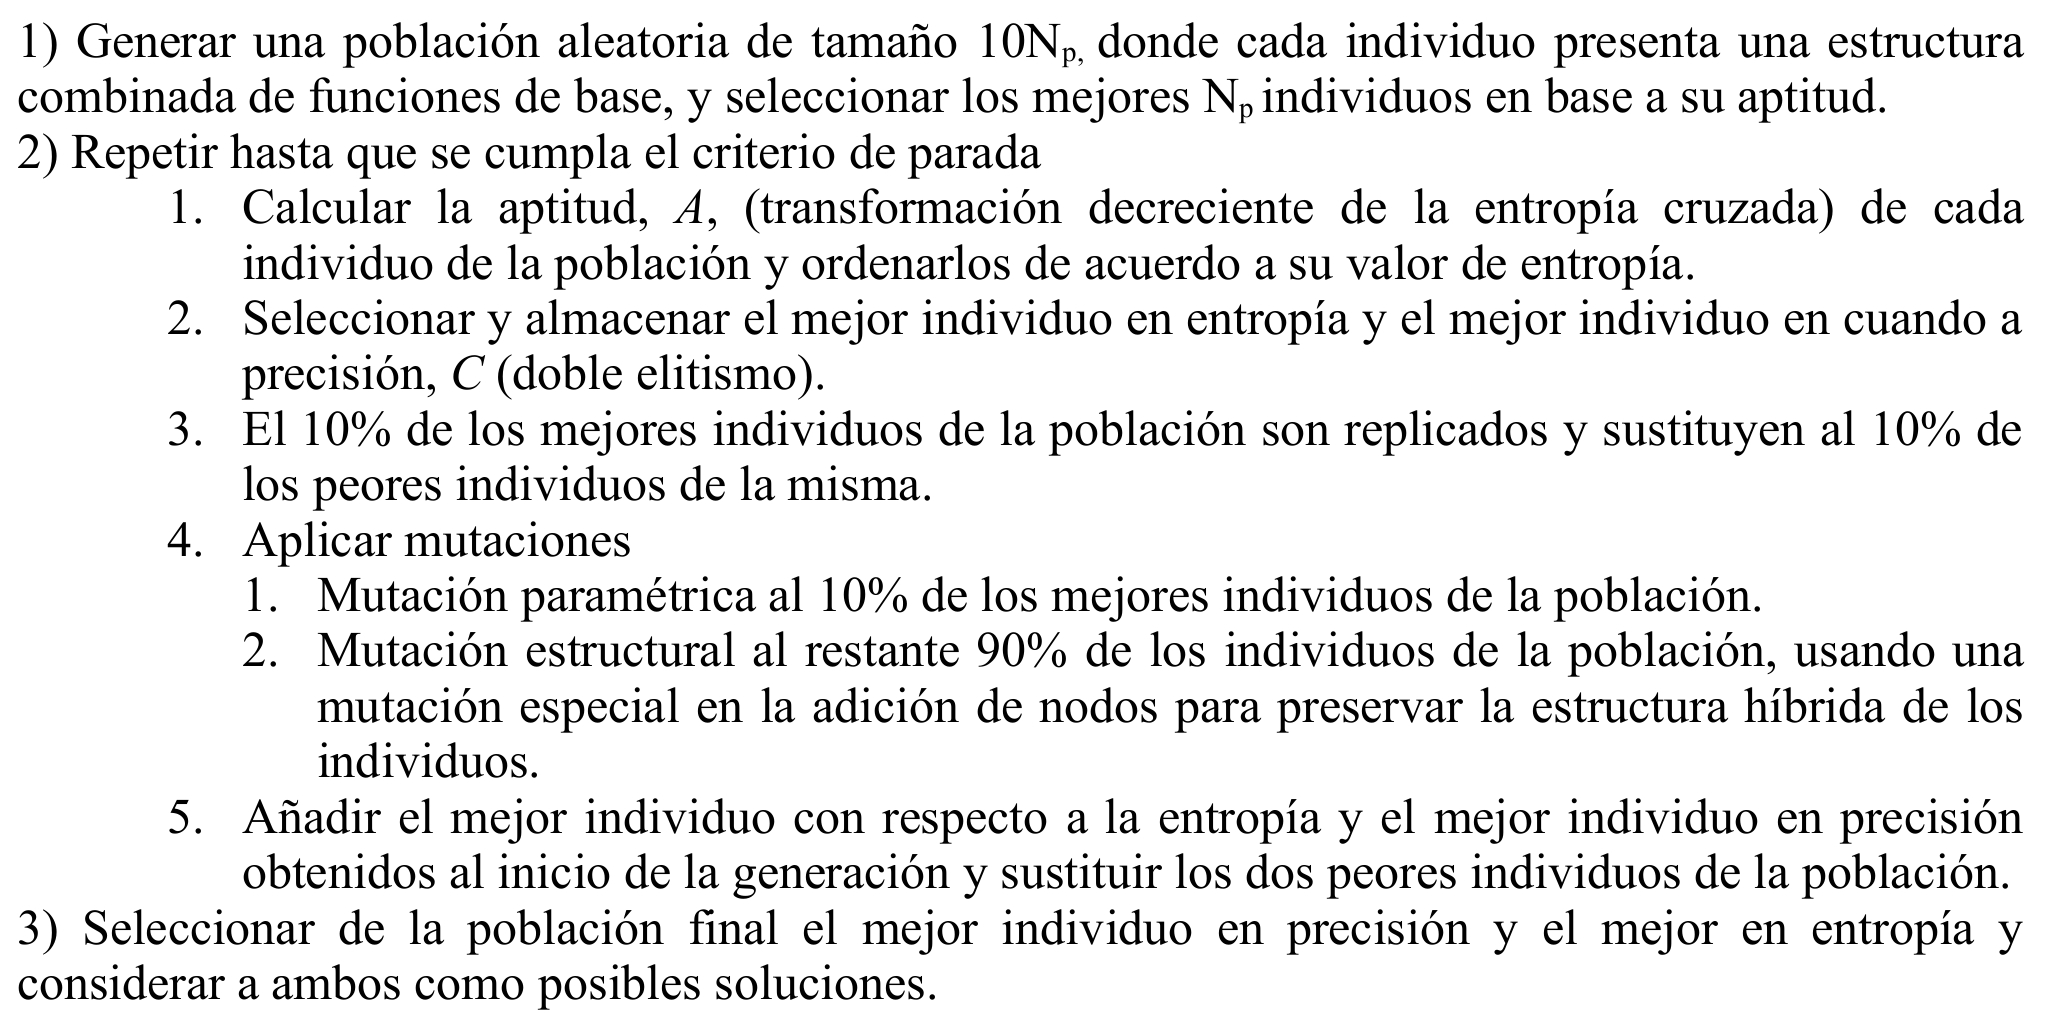
\includegraphics[keepaspectratio,width=12.5cm]{figuras/marcoNNEP.jpg}
}
\caption{Marco general del algoritmo CBFEP.}
\label{marcoNNEP}
\end{figure}
\begin{figure}[htb]
\centering
	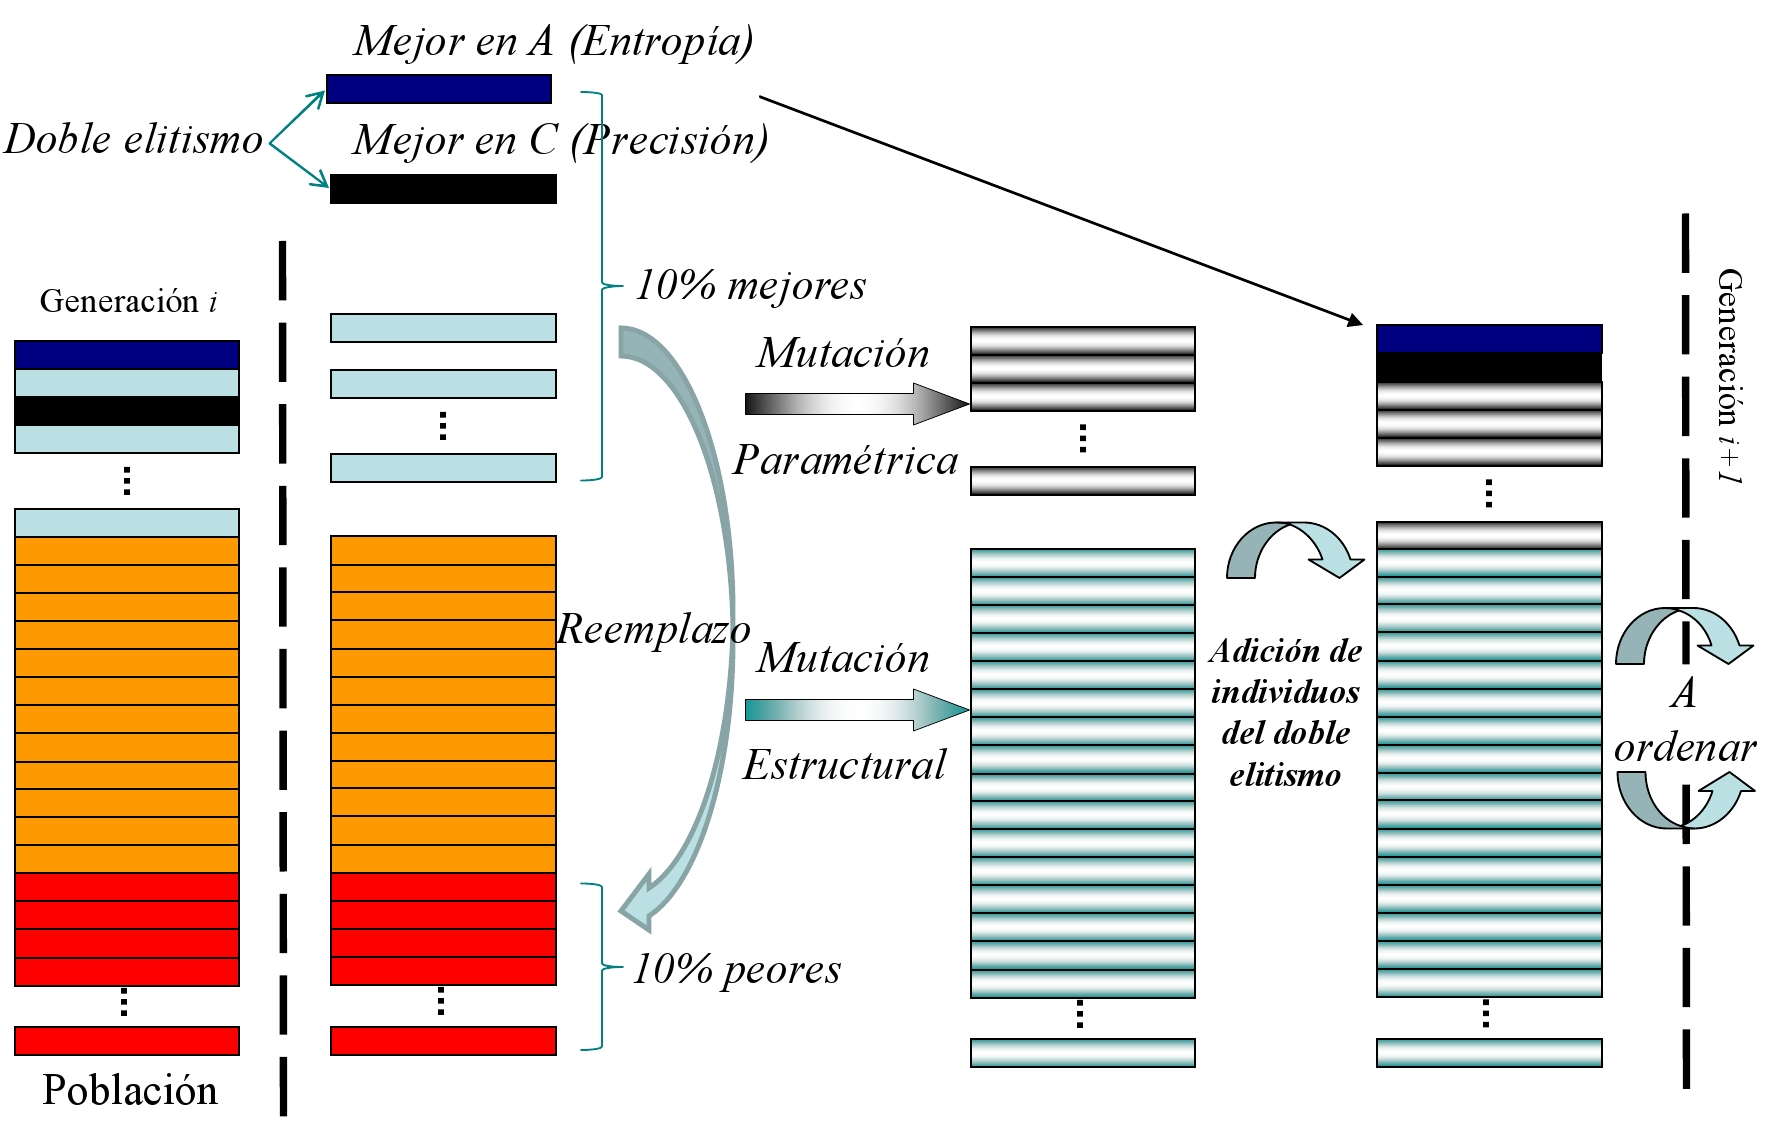
\includegraphics[keepaspectratio,width=12.5cm]{figuras/etapasNNEP.jpg}
\caption{Esquema del procedimiento de doble elitismo.}
\label{etapasNNEP}
\end{figure}
\newpage
\subsection{Función objetivo}
\noindent La función de aptitud que usamos con el algoritmo CBFEP, es una transformación
estrictamente decreciente de la función de entropía cruzada, $E$, comentada en la sección
\ref{metricasmulticlase} del capítulo
\ref{medidasRendimiento}. Teniendo en cuenta el modelo funcional asociado a las redes
híbridas y a la función $E$, la aptitud viene dada por:
\begin{equation}\label{aptitudNNEP}
A\left( g,\mathbf{\Theta}\right) =\frac{1}{1+E\left( g,\mathbf{\Theta}\right)}
\end{equation}
Una ventaja de utilizar $E$ y no $(1-C)$ (como podría pensarse), es que $E$ es una función
continua, lo que hace que la convergencia sea más robusta. En varios estudios se ha
demostrado
que $E$, por norma general, tiene mayor robustez que $C$ en problemas de clasificación
\cite{Bishop1995,Bishop2006}.

\subsection{Operadores}\label{operadores}
\noindent Antes de comenzar a describir el algoritmo, describiremos los operadores
de mutación utilizados en CBFEP durante el proceso evolutivo. Estos se dividen en
mutaciones estructurales y una mutación paramétrica.

Las mutaciones estructurales constan de 5 tipos:
% \begin{itemize}
% 	\item \textbf{Añadir neurona, (\textit{Add Neuron}, AN):} Consiste en añadir
% neuronas a
% la red.
% 	\item \textbf{Eliminar neurona, (\textit{Delete Neuron}, DN):} Consiste en eliminar
% neuronas	de la red.
% 	\item \textbf{Añadir enlace, (\textit{Add Link}, AL):} Consiste en añadir nuevos
% enlaces
% a la	red.
% 	\item \textbf{Eliminar enlace, (\textit{Delete Link}, DL):} Consiste en
% eliminar enlaces
% de la	red.
% 	\item \textbf{Unir neuronas, (\textit{Fusion Neurons}, FN):} Consiste
% en la unión o
% fusión de dos nodos de la red.
% \end{itemize}
\begin{description}
\item [Añadir neurona, (\textit{Add Neuron}, AN):] Consiste en añadir neuronas a la red.
\item [Eliminar neurona, (\textit{Delete Neuron}, DN):] Consiste en eliminar neuronas	de
la red.
\item [Añadir enlace, (\textit{Add Link}, AL):] Consiste en añadir nuevos enlaces a la
red.
\item [Eliminar enlace, (\textit{Delete Link}, DL):] Consiste en eliminar enlaces de la
red.
\item [Unir neuronas, (\textit{Fusion Neurons}, FN):] Consiste en la unión o fusión de dos
nodos de la red.
\end{description}

Según el paso 4.2 de la figura \ref{marcoNNEP}, al 90\% de los individuos de la
población se le aplica una de las 5 mutaciones estructurales comentadas anteriormente.
Para ello disponemos de un valor de temperatura $T$ que posee cada individuo en base a su
aptitud, y que viene dado por $\displaystyle T(g)= 1-A(g)$. Aleatoriamente se escoge un
valor entre $\left[0,1\right]$, y si ese valor es menor que $T$, se aplica la primera de
las 5 mutaciones estructurales existentes en este orden: AN-DN-AL-DL-FN, de forma que si
la mutación ha sido exitosa el proceso de mutación del individuo termina. Si el valor
aleatorio es mayor que $T$, o por circunstancias especiales de topología, (no tener nodos
en capa oculta, que una neurona se quede sin conexiones o sin enlace a la capa de salida,
o que se sobrepase el número máximo de nodos establecidos ``a priori``, etc), la mutación a
aplicar no pudiera utilizarse (mutación no exitosa), se procedería del mismo modo a
aplicar el siguiente tipo de mutación de la lista, según el orden establecido. Si ninguna
mutación tiene éxito, se elige de manera forzosa y aleatoriamente cualquiera de las
mutaciones anteriores, siempre que no conlleve ninguna situación especial de la topología
de la red. A medida que nos aproximamos al final del proceso evolutivo,
la probabilidad de mutar a un individuo es menor, ya que su aptitud aumenta.

Las mutaciones AL y DL se aplican solamente en la capa oculta y en la
capa de salida, mientras que las mutaciones AN, DN y FN se
realizan en capa oculta. El número de neuronas a añadir o eliminar se elije
aleatoriamente entre los valores $\left[1,2\right] $, mientras que el número de enlaces a
añadir o eliminar depende del que haya en ese momento en cada red. Se añadirán o
eliminarán el 30\% del total
de enlaces que haya entre capa de entrada y capa oculta y el 5\% del total de los enlaces
existentes entre capa oculta y capa de salida.

\subsubsection{Mutación añadir neurona}
\noindent A la hora de añadir neuronas se hace tantas veces como número de neuronas
tengamos que añadir (depende del valor aleatorio obtenido). También se elegirá
aleatoriamente el tipo de unidad de base. Si una neurona no puede añadirse porque la capa
oculta ya posee el número máximo de neuronas posibles y establecidas al comienzo del
proceso evolutivo (ver subsección \ref{etapas}), la mutación se dará por no exitosa. En
caso de que el número de neuronas a añadir fueran dos y la primera si se hubiese añadido,
pero la segunda no, la mutación se dará por exitosa, es decir, con una sola adición de
neurona la mutación ya se considera correcta.

En cuanto a los pesos de los enlaces asociados a las neuronas añadidas, se establecen de
la siguiente manera:
\begin{itemize}
	\item Enlaces con la capa de entrada: El número de enlaces de entrada a añadir a la
	nueva neurona se escoge aleatoriamente en el intervalo definido por $\left[
	1,numeroEntradas\right]	$. El peso asignado a cada enlace es el mismo con el que se
	crean las redes al inicio del	proceso evolutivo, es decir, un valor aleatorio entre
	$\left[-1,1\right]$, pero es configurable. Para cada	enlace, la neurona de entrada
	se escoge aleatoriamente, y se añade, exista	o no. Si	existe se sobre-escribe su
valor.
	\item Enlaces con la capa de salida: El número de enlaces de salida a añadir a la
	nueva neurona se escoge aleatoriamente en el intervalo $\left[ 1,numeroSalidas\right]$.
	El peso asignado a cada enlace es el mismo con el se crean las redes al
	inicio, un valor aleatorio entre $\left[ -10,10\right] $, pero este parámetro es
	configurable. Para
	cada enlace, la neurona de salida se escoge aleatoriamente. En este caso, si se evita
	el sobre-escribir un enlace añadido anteriormente ya que su comprobación es menos
	costosa	computacionalmente porque que el número de neuronas de salida (número de
	clases) suele ser menor	que el de neuronas de entrada (número de atributos).
\end{itemize}

\subsubsection{Mutación eliminar neurona}
\noindent Se elige aleatoriamente la neurona que será eliminada, y se hace tantas veces
como numero de neuronas haya que eliminar, dependiendo del valor aleatorio obtenido. Si al
intentar borrar una neurona, la capa oculta ya posee el número mínimo de neuronas
establecidos al inicio del proceso evolutivo, se termina este tipo de mutación y se pasa a
al siguiente tipo. En caso de que el número de neuronas a eliminar fueran dos y la primera
sí se hubiese eliminado pero la segunda no, la mutación se dará por exitosa. Otro caso con
el que hay que tener especial cuidado es si la neurona escogida para eliminar, es la única
neurona con la cual está enlazada una neurona de capa de salida, entonces la neurona no se
elimina y se elige aleatoriamente otra sin tener en cuenta la anterior. Esto sirve para
evitar que en capa de salida nos aparezca una neurona que no tenga enlaces con ninguna
neurona de la capa oculta, o sólo tenga enlace con la neurona que representa el sesgo. Con
respecto a los enlaces asociados a la neurona/s eliminada/s, éstos también se eliminan.

\subsubsection{Mutación añadir enlace}
\noindent Se elige aleatoriamente la neurona de la capa que será mutada (neurona destino
del enlace) y la neurona de la capa anterior desde la cual añadiremos el enlace (neurona
origen del enlace). Esta mutación se hace
tantas veces como número de enlaces tengamos que añadir, según el total de enlaces que hay
entre capa oculta y capa de entrada y entre capa de salida y capa oculta. Si el enlace ya
existiese antes de aplicar la mutación, el enlace será sobre-escrito con el nuevo valor
del peso. Por tanto, esta mutación siempre tiene éxito.

\subsubsection{Mutación eliminar enlace}
\noindent El proceso de eliminación a la hora de escoger un enlace es el mismo que en la
mutación AL, pero teniendo en cuenta los siguientes casos especiales: Si el
enlace elegido es el único de la neurona destino, no se elimina. Si la neurona destino es
la neurona de salida y, aunque ésta tenga más enlaces, al quitarlo provocásemos que la
neurona oculta origen se quedase sin ningún enlace de salida, no se elimina. En estos
casos la mutación no tiene éxito.

\subsubsection{Mutación unir neuronas}
\noindent La mutación FN consiste en elegir aleatoriamente dos neuronas \textit{a} y
\textit{b}, y sustituirlas por otra nueva neurona \textit{c}. Si la capa oculta ya posee el
número mínimo de neuronas preestablecido, la mutación no tiene éxito (se pasaría al
siguiente tipo de mutación). Si la capa oculta es híbrida, las neuronas elegidas deben ser
del mismo tipo. Si no hay dos neuronas del mismo tipo, la mutación no tiene éxito(se
pasaría al siguiente tipo de mutación). Se conservarán los enlaces en la neurona \textit{c}
con los nodos comunes a las neuronas \textit{a} y \textit{b}, y también se conservan con
una probabilidad de $0.5$ los que no sean comunes. El resultado de la fusión queda así
(ver ejemplo en figura \ref{unirNodos}):
\begin{itemize}
\item Enlaces de entrada de la nueva neurona resultado de la unión: Por cada entrada, si
ambas neuronas originales poseían ese enlace de entrada, el enlace se conserva con un peso
igual a la media de ambos pesos. Si sólo una neurona poseía ese enlace de entrada, el
enlace se conserva con una probabilidad de $0.5$ y con el mismo peso. Si ninguna neurona
poseía ese enlace de entrada, la neurona resultado tampoco lo poseerá.
\item Enlaces de salida de la nueva neurona resultado de la unión: Por cada neurona de
salida, si ambas neuronas originales poseían ese enlace de salida, el enlace se conserva
con un peso igual a la suma de ambos pesos. Si sólo una neurona poseía ese enlace de
salida, el enlace se conserva con una probabilidad de $0.5$ y con el mismo peso. Si
ninguna neurona poseía ese enlace de salida, la neurona resultado tampoco lo poseerá.
\begin{displaymath}
u_{i}^c=\frac{u_{i}^a+u_{i}^b}{2}; \quad w_{i}^c=\frac{w_{i}^a+w_{i}^b}{2}; \quad
\alpha_{j}^c=\alpha_{j}^a+\alpha_{j}^b; \quad \beta_{j}^c=\beta_{j}^a+\beta_{j}^b
\end{displaymath}
para $i$ igual al número de neuronas en capa oculta y $j$ igual al número de neuronas en
capa de salida.
\end{itemize}

\begin{figure}[htb]
\centering
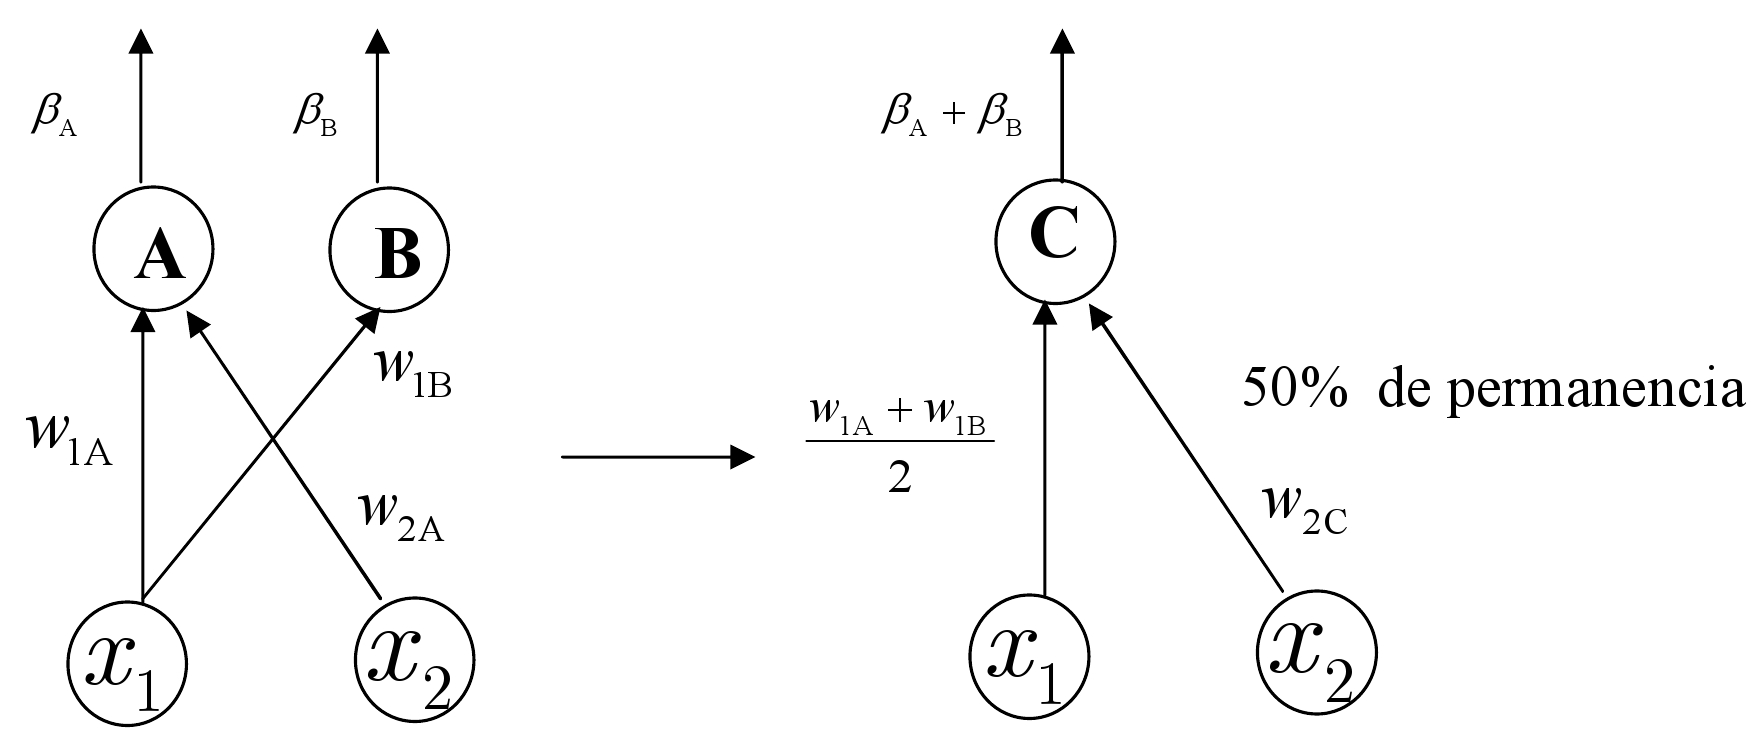
\includegraphics[keepaspectratio,width=10.5cm]{figuras/unirNodos.jpg}
\caption{Ejemplo de fusión de dos neuronas con la mutación FN.}
\label{unirNodos}
\end{figure}

En el caso de las neuronas RBF, la unión debe hacerse de otro modo, ya que el
significado de dichas neuronas es diferente, encargándose cada una de modelar una zona del
espacio cercana a su centro. El hecho de que las funciones combinadas puedan
interpretarse
como circunferencias de centro y radio perfectamente identificados obliga a que, al
combinar ambas neuronas, se tenga en cuenta este conocimiento topológico. Llamemos $
\mathbf{c}_j$ al centro definido por la neurona $j$, es decir,
$(w_{1j},w_{2j},...,w_{kj})$ y $r_j$
a su radio. En este caso, la mutación FN de dos neuronas RBF, $a$ y $b$,
consistirá en calcular el centro y radio de la neurona $c$ como:
\begin{center}
$\mathbf{c}_{c} =
$\begin{Large}$\frac{r_a}{r_a+r_b}$\end{Large}$\cdot \mathbf{c}_a
+$ \begin{Large}$\frac{r_b}{r_a+r_b}$\end{Large}$\cdot \mathbf{c}_b$
$\quad r_{c}=$\begin{Large}$\frac{r_a +
r_b}{2}$\end{Large}
\end{center}

\subsubsection{Mutación paramétrica}
\noindent La mutación paramétrica consiste en la alteración de todos los pesos de
la red (el sesgo también se muta paramétricamente), sumando un ruido gaussiano, donde la
varianza de la distribución de Gauss depende de la temperatura, $T$, definida
anteriormente. De esta forma, al principio del EA, cuando el proceso de
búsqueda se está iniciando, la aptitud de la red es cercana a cero y por tanto la
temperatura es alta, por lo que las mutaciones
son más grandes. A medida que nos acercamos al final del proceso evolutivo, disminuye la
temperatura, por lo que los cambios que se realizan en los pesos de las redes van siendo
más pequeños, afinando así la búsqueda.

Si consideramos el modelo funcional de la sección \ref{redesHibridas} del capítulo
\ref{redesneuronales}, los pesos de la capa intermedia quedarían
actualizados de la siguiente forma:
\begin{center}
$u_{ij}(t+1) = u_{ij}(t)+\xi_1(t)$\\
$w_{ij}(t+1) = w_{ij}(t)+\xi_1(t)$\\
$\theta_j(t+1) = \theta_{j}(t)+\xi_2(t)$\\
\end{center}
para $i$ igual al número de neuronas en capa de entrada y $j$ igual al número de neuronas
en capa de oculta, siendo $\xi_1(t)$ y $\xi_2(t)$ un valor aleatorio de la
distribución normal $N(0, \alpha_1(t)T(t))$, donde $\alpha_1(t)$ es un parámetro que junto
con la temperatura determina la varianza de la distribución, la cual varía durante la
evolución adaptando el proceso de aprendizaje, y $t$ el número de generación donde
se encuentra el EA.

Siguiendo esta misma filosofía, si la neurona a mutar es una unidad RBF, la
actualización del radio viene dada por $r_{j}(t+1) = r_j(t)+\xi_1(t)$.

En cuanto a los pesos de la capa de salida se actualizarán de forma análoga:
	\begin{center}
	$\alpha_{ij}(t+1) = \alpha_{ij}(t)+\xi_2(t)$\\
   $\beta_{ij}(t+1) = \beta_{ij}(t)+\xi_2(t)$\\
   \end{center}
para $i$ igual al número de neuronas en capa de salida y $j$ igual al número de
neuronas	en capa de oculta, y siendo $\xi_2(t)$ un valor aleatorio de la distribución
normal $N(0, \alpha_2(t)T(t))$, donde $\alpha_1(t)$ es un parámetro que junto con la
temperatura determina la varianza de la distribución, la cual varia durante la evolución
adaptando el proceso de aprendizaje. Se
cumple además que $\alpha_1(t) << \alpha_2(t)$,  es decir,   las mutaciones de los pesos
$w_{ij}$ y $\theta_j$,   correspondientes a los pesos con que se ponderan las variables
de la función que queremos modelar, han de ser menores que las   mutaciones realizadas en
los pesos $\beta_{ij}$,   correspondientes a los coeficientes de las unidades de base de
la función. Esto se debe a que el efecto de una mutación de un   peso que pondera a una
variable de entrada es mucho mayor que   el de un coeficiente, y por lo tanto los cambios
a realizar   deben ser menores.

Una vez realizado el cambio en el espacio de los pesos, la aptitud del individuo se
recalcula y se aplica un   algoritmo estándar de enfriamiento simulado. Si llamamos
$\triangle A$ a la variación de la aptitud antes y después del   cambio en los pesos,
resulta que:
   \begin{itemize}
   \item[-] Si $\triangle A\geq 0$, se acepta el cambio.
   \item[-] Si $\triangle A<0$, se acepta el cambio
   si \begin{Large}$e^{\frac{\triangle A}{T}}$\end{Large}
   $<\gamma$, donde $\gamma \in U(0,1)$
   \end{itemize}

Los parámetros $\alpha_1$ y $\alpha_2$  van cambiando durante el proceso de evolutivo
(al   contrario que la versión estática en \cite{Angeline1994}),   realizando en este
sentido un aprendizaje adaptativo. De esta   forma evitamos quedar atrapados en mínimos
locales y aceleramos		el proceso de evolución cuando las condiciones del proceso lo
permiten. Se debe escoger un mecanismo de evolución de los parámetros
$\alpha_1$ y $\alpha_2$ que converja más rápido hacia los      valores óptimos. El
mecanismo escogido en este caso es la regla  de razón de éxito 1/5 de Rechenberg, uno
de los métodos más simples. Según esta regla, la razón de mutaciones satisfactorias
debería ser siempre 1/5 \cite{Rechenberg1973}. De esta forma, si la razón es mayor que 1/5
la varianza debería incrementarse; en caso contrario,  debería disminuirse. Esto es:
      \begin{center}
      $
      \begin{array}{c} \\ \alpha_i(t+s) \\ i=1,2 \end{array} =
      \left\{
			\begin{array}{ccl}
         (1+\beta)\alpha_i(t), & & si \enskip s_g>1/5 \\
         (1-\beta)\alpha_i(t), & & si \enskip s_g<1/5 \\
         \alpha_i(t),  & & si \enskip s_g=1/5 \\
         \end{array}
         \right.
         $
         \end{center}
siendo $s_g$ la razón de mutaciones satisfactorias durante $s$ generaciones. En todos los
experimentos realizados con el algoritmo CBFEP hemos tomado un valor de $\beta=0.1$ y
un valor de $s$ igual a 5, $\alpha_{1}(0)=1$ y $\alpha_{2}(0)=5$.

\subsection{Etapas y aspectos relevantes de CBFEP}\label{etapas}
\noindent Una vez descritos los operadores de mutación, pasamos a comentar algunos de los
aspectos más relevantes del mismo, y las etapas o bloques usados para la obtención de
modelos de red híbridos.

CBFEP comienza con la generación aleatoria de una
población inicial de redes híbridas, haciéndolas evolucionar utilizando diferentes
mutaciones y operaciones de replicación. El modelo funcional de cada red híbrida es el
expuesto en la sección \ref{redesHibridas} del capítulo \ref{redesneuronales}. La
población inicial que se genera es de tamaño $10N_{p}$, donde $N_{p}=1000$ es el tamaño de
la población durante el proceso evolutivo. Entonces se seleccionan las mejores $N_{p}$
redes en base a su aptitud.

El enfoque adoptado a la hora de interpretar la salida de una ANN es  un
enfoque probabilístico. Consideramos un esquema de codificación ``1 de $Q$'', siendo $Q$
el número de clases del problema. Una nueva observación se asigna a la clase
correspondiente al valor de salida más grande de cada una de las neuronas que componen la
capa de salida (existe una neurona por cada clase). Ese valor es calculado en base a la
función \textit{softmax}, que viene dada por la siguiente expresión:
\begin{displaymath}
g_{q}(\mathbf{x})=\frac{exp^{f_{q}(\mathbf{x})}}{\sum_{i=1}^{Q} exp^{f_{q}(\mathbf{x})}}
\end{displaymath}
donde $Q$ es el número de clases del problema, $f_{q}(\mathbf{x})$ se corresponde con la
función de salida de la neurona $q$ descrita en la sección \ref{modelos} del capítulo
\ref{redesneuronales}, y $g_{q}(\mathbf{x})$ es la probabilidad de que el patrón
$\mathbf{x}$
pertenezca a la clase $q$. La  transformación  \textit{softmax}  produce estimaciones
positivas en todas las salidas, de forma que la suma de todas ellas es uno, lo que hace
que  las  salidas  puedan  ser interpretadas  como  la  probabilidad  de  pertenencia  a
la  clase correspondiente. Expresado formalmente esta definición viene dada por:
\begin{displaymath}
R(\mathbf{x})= \hat{q} \quad \text{donde} \quad \hat{q}=\text{arg} \: max_{i}\:
g_{i}(\mathbf{x})
= max_{i}\:f_{i}(\mathbf{x})
\end{displaymath}

Al  tratarse  de  probabilidades  de  pertenencia  a  una  clase,  está  claro  que  no
es  necesario calcularlas todas, ya que la última probabilidad $g_{Q}(\mathbf{x})$ se
puede
calcular en función del resto como $\displaystyle 1-\sum_{i=1}^{Q-1}g_{i}(\mathbf{x})$. De
esta  forma,  podemos  simplificar  el  modelo  definiendo  la  salida  de  una de  las
neuronas de la capa de salida con un valor constante e igual a 0, es decir,
$\displaystyle f_{Q}(\mathbf{x})=0$.

Una característica específica de este algoritmo es el doble elitismo. CBFEP
devuelve el mejor individuo en $E$ y el mejor individuo en $C$, (paso 3 de la
figura \ref{marcoNNEP}); así consideramos también los casos en los que se obtengan
mejores individuos utilizando $C$ y no $E$. Esto se consigue evaluando a los individuos
de la población usando $A$ como aptitud y obteniendo el número de patrones correctamente
clasificados para cada uno de ellos (todo en el conjunto de entrenamiento). En general,
la relación entre $E$ y $C$ depende fuertemente de la estructura del conjunto de datos,
por lo que en ocasiones, el uso de $E$ hará que se obtengan mejores
resultados en $C$ sobre el conjunto generalización, mientras que otras veces, se
obtendrán mejores resultados con el uso directo de $C$. Por esta razón se contemplan ambos
casos como evaluadores de los modelos de red.

Siguiendo las etapas del algoritmo, una vez creada la población y evaluados los
individuos en función de $A$, en la generación $i$ se almacenan el mejor individuo en $A$
y en $C$ (paso 2.2 de la figura \ref{marcoNNEP}). Entonces se aplica un proceso de
selección y reemplazo (sin tener en cuenta los dos individuos elitistas), que usa el 10\%
de los mejores individuos de la población y los sustituye por el 10\% peores (paso 2.3 de
la figura \ref{marcoNNEP}). Una vez hecho esto se realiza una mutación paramétrica al 10\%
de los mejores individuos (sin tener en cuenta los dos mejores individuos seleccionados
previamente), y una mutación estructural al 90\% restante (paso 2.4 de la figura
\ref{marcoNNEP}). Finalmente, la población se evalúa y se forma la siguiente
generación, añadiendo los individuos almacenados en el doble elitismo, concretamente
reemplazando a los dos peores (paso 2.5 de la figura \ref{marcoNNEP}) y ordenando la
población en función de $A$. El proceso continua volviendo al paso 2.1 de la figura
\ref{marcoNNEP}.

Con respecto a la optimización de la estructura de las redes híbridas durante el proceso
evolutivo, se consideran tres parámetros: $m$, $M_{E}$ y $M_{I}$, correspondientes al
mínimo y máximo número de nodos ocultos en el proceso evolutivo y al máximo número de
nodos ocultos en el proceso de inicialización respectivamente. Para comenzar con unos
modelos de red más simples que la máxima complejidad posible establecida, se debe fijar la
condición $m\leq M_{I} \leq M_{E}$. Para la generación de una red, el número de
nodos en capa oculta se elige en base a una distribución uniforme $\left[
m,M_{I}\right]$. Una vez que se decide el número de neuronas, cada nodo oculto se genera
con una probabilidad de $0.5$ para decidir si el nodo se corresponde con un tipo de nodo
$B_{1}$ o $B_{2}$. Para nodos PUs o SUs, el número de conexiones entre
cada nodo de la capa oculta y los nodos de entrada, se determina a partir de una
distribución
uniforme en el intervalo $\left[ 0,k\right]$, donde $k$ es el número de variables
independientes. Para nodos ocultos RBF el número de conexiones es siempre $k$, ya
que estas conexiones representan las coordenadas del centro del nodo. El número de
conexiones entre cada nodo oculto y la capa de salida se determina a partir de una
conexión uniforme en el intervalo $\left( 0,Q-1\right)$.

Los pesos se inicializan de manera diferente dependiendo del tipo de nodo oculto
generado. Para nodos PUs y SUs, los pesos se asignan en función de una
distribución uniforme en dos intervalos: $\left[ -5,5\right] $ para las conexiones entre
capa de entrada y capa oculta, para ambos tipos de nodos, y $\left[ -10,10\right] $
para conexiones entre la capa oculta y la capa de salida. Para nodos ocultos RBF
las conexiones entre la capa de entrada y la capa oculta representan el centro de la
distribución Gausiana asociada, y estos centros se inicializan usando un algoritmo de
clustering, de manera que el EA puede comenzar el proceso evolutivo con los
centros bien posicionados. La idea es agrupar los datos de entrada en $k$ grupos, siendo
$k$ el numero de nodos ocultos RBF. De esta forma cada nodo oculto se puede
posicionar en el centroide de su correspondiente grupo. Finalmente el radio de los nodos
RBF se calcula como la media geométrica de la distancia a los dos centroides más
cercanos. La técnica de agrupamiento utilizada (similar a la propuesta por Cohen e
Intrator \cite{Coen2000}) es una modificación del algoritmo clásico ``k-medias``, donde
los centroides iniciales se calculan usando una inicialización específica del algoritmo
que evita los mínimos locales, incrementando la probabilidad de que los centros de las
$k$ agrupaciones iniciales no provengan de un número de agrupaciones más pequeño.

Por último, la condición de parada de CBFEP se cumple cuando se den una de estas
dos condiciones:
\begin{itemize}
\item Que se alcance un número de generaciones sin mejorar la media de aptitud del 10\%
de los mejores individuos y la aptitud del mejor individuo.
\item Que se alcance un número máximo de generaciones establecido.
\end{itemize}

\subsection{Diseño experimental}
\noindent Para analizar el rendimiento de CBFEP hemos utilizado 10
bases de datos del repositorio de la UCI \cite{UCI2007}, analizando
los resultados obtenidos tanto para modelos puros como híbridos. Como nuestro
procedimiento es estocástico, utilizamos un diseño experimental que consiste en una
partición
estratificada del
conjunto de datos con $3n/4$ patrones para el conjunto de entrenamiento y $n/4$ patrones para el
conjunto de generalización, siendo $n$ el tamaño del conjunto.

Todos los parámetros de CBFEP son comunes a los 10
experimentos, excepto $m$,
$M_{I}$, $M_{E}$ y el número de generaciones usadas. Estos valores, junto con las
características de cada base de datos, se representan en la tabla \ref{tabla1NNEP}.

\begin{table}[htb]
\caption{Características principales de cada base de datos y valor de parámetros no
comunes.}
\label{tabla1NNEP}
\centering
\tabcolsep 1pt
\begin{tabular}{ccccccccc} \hline
\rowcolor[rgb]{0.70,0.85,1} \textbf{B. datos} & \textbf{Instancias} &
\textbf{Entradas} &
\textbf{Distribución} & \textbf{Clases} & \textbf{Gen.} & $\mathbf m$ & $\mathbf
M_{I}
$ & $\mathbf M_{E} $ \\ \hline
\rowcolor[rgb]{0.86,0.94,1}Balance & 625 & 4 & (288,49,288) & 3 & 500 & 3 & 4 & 5 \\
\rowcolor[rgb]{0.86,0.94,1}Card & 690 & 51 & (307, 383) & 2 & 50 & 1 & 2 & 3 \\
\rowcolor[rgb]{0.86,0.94,1}German & 1000 & 61 & (700,300) & 2 & 300 & 2 & 3 & 4 \\
\rowcolor[rgb]{0.86,0.94,1}Glass & 214 & 9 & (17,76,13,29,70,9) & 6 & 500 & 7 & 8 & 9 \\
\rowcolor[rgb]{0.86,0.94,1}Heart & 270 & 13 & (150,120) & 2 & 100 & 1 & 1 & 2 \\
\rowcolor[rgb]{0.86,0.94,1}Ionosphere & 351 & 34 & (126,225) & 2 & 300 & 3 & 4 & 5 \\
\rowcolor[rgb]{0.86,0.94,1}Newthyroid & 215 & 5 & (150,35,30) & 3 & 100 & 1 & 1 & 4 \\
\rowcolor[rgb]{0.86,0.94,1}Pima & 768 & 8 & (500,268) & 2 & 160 & 1 & 2 & 3 \\
\rowcolor[rgb]{0.86,0.94,1}Vote & 435 & 16 & (267,168) & 2 & 10 & 1 & 1 & 2 \\
\rowcolor[rgb]{0.86,0.94,1}Zoo & 101 & 16 & (41,20,5,13,4,8,10) & 7 & 400 & 2 & 3 & 3 \\
\hline
\end{tabular}
\end{table}

\subsection{Resultados}
\noindent En cuanto a los resultados experimentales obtenidos, la tabla \ref{tabla2NNEP} muestra la
media y la desviación típica para los valores de
precisión en generalización, $C_{G}$, y la media y la desviación típica del número de
enlaces o conexiones de los mejores modelos obtenidos en 30 ejecuciones del algoritmo.
Como CBFEP devuelve de manera conjunta el mejor individuo en $C$ y en $E$, se
muestran dos medias y dos desviaciones típicas. Para reducir la extensión de la tabla, los
resultados incluidos corresponden solo a la variante con los mejores resultados en cada
modelo, ya que la idoneidad de cada elitismo depende de las características de la
base de datos y de la estructura de la función de base utilizada. Podemos observar que la
combinación de funciones de base obtiene buenos resultados en $C_{G}$. Desde un punto de
vista puramente descriptivo, hemos obtenido los mejores resultados en seis
de las diez
bases de datos utilizando modelos híbridos, y los segundos mejores resultados en tres
de las cuatro bases de datos restantes.

\begin{table}[htb]
\scriptsize
\caption{Resultados estadísticos en $C_{G}$ (generalización) y número de
enlaces en 30 ejecuciones, utilizando funciones de base puras e híbridas. Se indica
el tipo de elitismo, mejor en precisión $(C)$ o en entropía $(E)$.}
\label{tabla2NNEP}
\centering
\tabcolsep 1pt
\begin{tabular}{cccccccccc} \hline
\rowcolor[rgb]{0.70,0.85,1}\textbf{B. datos} & \textbf{Func.} & \textbf{Elit.} &
$\mathbf {C_{{\mathbf\rm G}}} $ & \textbf{Enlaces} & \textbf{B. datos} &
\textbf{Func.} & \textbf{Elit.} & $\mathbf {C_{{\mathbf\rm G}}} $ & \textbf{Enlaces}
\\
\rowcolor[rgb]{0.70,0.85,1}&  &  & \textbf{Media$\pm$SD} & \textbf{Media$\pm$SD} &  &  &
 & \textbf{Media$\pm$SD} & \textbf{Media$\pm$SD} \\ \hline
\rowcolor[rgb]{0.86,0.94,1}Balance & PU & C & 96.45$\pm$1.28 & 23.1$\pm$2.6 & Card & PU &
E & 87.50$\pm$2.75 & 24.6$\pm$14.7 \\
\rowcolor[rgb]{0.86,0.94,1}& SU & C & 95.11$\pm$1.58 & 31.9$\pm$1.8 &  & \textit{SU} & E &
\textit{87.71$\pm$1.42} & 52.1$\pm$10.8 \\
\rowcolor[rgb]{0.86,0.94,1}& RBF & C & 90.77$\pm$1.31 & 29.7$\pm$3.0 &  & RBF & C &
76.69$\pm$3.33 & 124.2$\pm$24.1 \\
\rowcolor[rgb]{0.86,0.94,1}& \textbf{PSU} & C & \textbf{98.01$\pm$0.96} & 29.3$\pm$4.5 &
& PSU & E & 87.38$\pm$1.17 & 43.3$\pm$15.9 \\
\rowcolor[rgb]{0.86,0.94,1}& \textit{PRBF} & C & \textit{97.41$\pm$1.11} & 26.6$\pm$3.9 &
& PRBF & C & 86.43$\pm$4.09 & 61.4$\pm$32.5 \\
\rowcolor[rgb]{0.86,0.94,1}& SRBF & C & 92.91$\pm$1.61 & 32.6$\pm$2.0 &  & \textbf{SRBF} &
E & \textbf{88.02$\pm$1.01} & 62.2$\pm$21.0 \\
\rowcolor[rgb]{0.86,0.94,1}German & PU & C & 71.24$\pm$1.52 & 47.9$\pm$19.5 & Glass & PU &
C & 65.16$\pm$4.17 & 62.4$\pm$7.1 \\
\rowcolor[rgb]{0.86,0.94,1}& SU & C & 73.07$\pm$1.64 & 93.9$\pm$21.8 &  & \textbf{SU} & E
& \textbf{67.67$\pm$3.49} & 83.8$\pm$6.0 \\
\rowcolor[rgb]{0.86,0.94,1}& RBF & C & 71.69$\pm$1.32 & 213.0$\pm$30.4 &  & RBF & C &
64.91$\pm$4.74 & 108.1$\pm$9.4 \\
\rowcolor[rgb]{0.86,0.94,1}& \textit{PSU} & E & \textit{73.12$\pm$1.71} & 86.0$\pm$21.9 &
& PSU & E & 66.23$\pm$3.91 & 82.8$\pm$6.5 \\
\rowcolor[rgb]{0.86,0.94,1}& PRBF & E & 71.25$\pm$1.45 & 119.6$\pm$43.9 &  & PRBF & C &
65.03$\pm$3.96 & 89.3$\pm$9.5 \\
\rowcolor[rgb]{0.86,0.94,1}& \textbf{SRBF} & E & \textbf{73.44$\pm$1.61} & 105.7$\pm$34.0
&  & \textit{SRBF} & C & \textit{67.17$\pm$4.36} & 97.9$\pm$7.5 \\
\rowcolor[rgb]{0.86,0.94,1}Heart & PU & C & 83.58$\pm$2.15 & 11.0$\pm$2.6 & Ionos & PU & E
& 91.15$\pm$2.20 & 39.1$\pm$9.8 \\
\rowcolor[rgb]{0.86,0.94,1}& \textbf{SU} & E & \textbf{86.91$\pm$2.06} & 17.2$\pm$2.0 &  &
\textit{SU} & E & \textit{92.61$\pm$1.56} & 73.9$\pm$10.2 \\
\rowcolor[rgb]{0.86,0.94,1}& RBF & C & 81.37$\pm$2.54 & 27.6$\pm$4.2 &  & RBF & C &
90.42$\pm$2.60 & 158.5$\pm$18.9 \\
\rowcolor[rgb]{0.86,0.94,1}& \textit{PSU} & C & \textit{85.93$\pm$2.27} & 16.9$\pm$2.6 &
& PSU & C & 92.11$\pm$1.88 & 67.9$\pm$12.6 \\
\rowcolor[rgb]{0.86,0.94,1}& PRBF & E & 82.79$\pm$2.57 & 20.4$\pm$4.4 &  & PRBF & E &
91.34$\pm$2.41 & 93.9$\pm$16.4 \\
\rowcolor[rgb]{0.86,0.94,1}& SRBF & E & 85.49$\pm$1.96 & 18.9$\pm$4.3 &  & \textbf{SRBF}
& C & \textbf{93.22$\pm$1.61} & 100.2$\pm$16.6 \\
\rowcolor[rgb]{0.86,0.94,1}Newth & \textit{PU} & C & \textit{96.85$\pm$2.71} &
16.4$\pm$3.2 & Pima & PU & E & 78.45$\pm$1.29 & 12.5$\pm$2.1 \\
\rowcolor[rgb]{0.86,0.94,1}& SU & C & 94.88$\pm$2.26 & 22.1$\pm$3.6 &  & \textbf{SU} & E
& \textbf{79.98$\pm$1.53} & 18.6$\pm$2.0 \\
\rowcolor[rgb]{0.86,0.94,1}& RBF & C & 95.00$\pm$2.01 & 24.2$\pm$3.8 &  & RBF & C &
75.66$\pm$2.56 & 26.8$\pm$3.1 \\
\rowcolor[rgb]{0.86,0.94,1}& PSU & E & 96.36$\pm$2.77 & 20.3$\pm$3.7 &  & PSU & E &
78.89$\pm$1.87 & 17.0$\pm$2.8 \\
\rowcolor[rgb]{0.86,0.94,1}& \textbf{PRBF} & E & \textbf{97.96$\pm$2.45 } & 19.7$\pm$3.8
&  & PRBF & E & 78.54$\pm$1.44 & 17.0$\pm$1.5 \\
\rowcolor[rgb]{0.86,0.94,1}& SRBF & C & 95.62$\pm$2.20 & 23.5$\pm$3.3 &  & \textit{SRBF}
& E & \textit{79.64$\pm$1.29} & 22.6$\pm$3.0 \\
\rowcolor[rgb]{0.86,0.94,1}Vote & \textit{PU} & E & \textit{95.52$\pm$2.26} & 5.9$\pm$2.4
& Zoo & \textbf{PU} & C & \textbf{94.80$\pm$4.48} & 29.7$\pm$2.8 \\
\rowcolor[rgb]{0.86,0.94,1}& SU & E & 94.26$\pm$1.91 & 14.0$\pm$4.5 &  & \textit{SU} & C
& \textit{92.67$\pm$4.34} & 49.9$\pm$4.5 \\
\rowcolor[rgb]{0.86,0.94,1}& RBF & C & 87.50$\pm$2.77 & 30.4$\pm$7.6 &  & RBF & C &
75.07$\pm$5.00 & 66.0$\pm$1.5 \\
\rowcolor[rgb]{0.86,0.94,1}& PSU & E & 94.57$\pm$1.96 & 12.8$\pm$4.3 &  & PSU & C &
92.13$\pm$5.09 & 42.2$\pm$6.8 \\
\rowcolor[rgb]{0.86,0.94,1}& \textbf{PRBF} & C & \textbf{96.02$\pm$0.88} & 13.3$\pm$8.2 &
 & PRBF & E & 91.33$\pm$5.95 & 35.3$\pm$6.0 \\
 \rowcolor[rgb]{0.86,0.94,1}& SRBF & C & 94.54$\pm$2.23 & 16.0$\pm$7.3 &  & SRBF & E &
90.40$\pm$4.77 & 48.6$\pm$5.2 \\ \hline
\multicolumn{10}{l}{El mejor resultado se indica en \textbf{negrita} y el segundo mejor en
\textit{cursiva}.
} \\
\end{tabular}
\end{table}

Para determinar estadísticamente las diferencias observadas en el rendimiento de cada
base de datos, hemos llevado a cabo un test de análisis de varianza ANOVA
(\textit{Analysis
of Variance}) \cite{Miller1996} para $C_{G}$ y para el número de enlaces
(previamente se ha evaluado si $C_{G}$ sigue una distribución normal usando un test de
Kolmogorov-Smirnof). Basado en la
hipótesis de normalidad, ANOVA examina los efectos de algunas variables
cualitativas (llamados factores) en una respuesta cuantitativa. El
objetivo de este análisis es estudiar si la influencia de las funciones de base usadas en
la capa oculta es significativa en media con respecto al $C_{G}$ obtenido por el
modelo de red. Así, el modelo
lineal para $C_{G}$ viene dado por $\displaystyle C_{G_{ij}}=\mu+B_{i}+e_{ij}$ para
$i=1,\cdots,6$ y $j=1,2,\cdots,30$. El factor $B_{i}$ analiza el efecto que tiene el
nivel $i-esimo$ del factor sobre la media de $C_{G}$, donde
$B_{i}$ representa la tipología de las funciones de base
usadas en la capa oculta de la red, con niveles: ($i=1$) para PUs; ($i=2$) para
SUs; (i=3) para RBFs; ($i=4$) para PSU; ($i=5$) para PRBF; ($i=6$) para SRBF. El término
$\mu$ es el efecto medio común
para todas las poblaciones. El término $e_{ij}$ es la influencia en el resultado de
factores aleatorios o de todos aquellos otros factores de los que no se conoce su efecto.

Para llevar a cabo el experimento se hicieron 180 simulaciones para cada base de datos,
correspondientes a las 30 ejecuciones de cada uno de los 6 niveles. Primero, se realizó un
test de Levene, \textit{L}, \cite{Levene1960} para evaluar la igualdad de las varianzas
(si $\alpha<\text{nivel crítico}$, entonces las varianzas de $C_{G}$ son iguales), y
después un test de
Snedecor \cite{Snedecor1980}, \textit{F}, para determinar si la influencia de la funciones de base
utilizadas
en capa oculta es significativa con respecto a $C_{G}$. El $\text{nivel crítico}$ de
ambos test se presenta en la tabla \ref{tabla3NNEP}. El test \textit{F} contrasta si la
tipología de las funciones de base utilizadas en la capa oculta presenta diferencias
significativas en media de $C_{G}$ en primer lugar, y en el número de enlaces de la red
en segundo lugar, para un nivel de significación $\alpha$ del 5\% (ver la tercera
columna, $\alpha>\text{nivel crítico}$ ).

\begin{table}[htb]
\caption{$\textbf{\text{Nivel crítico}}$ del test \textit{L} y el test \textit{F} de ANOVA
I
aplicado a $C_{G}$ y número de enlaces.}
\label{tabla3NNEP}
\centering
\begin{tabular}{ccccc} \hline
\rowcolor[rgb]{0.70,0.85,1} & \multicolumn{4}{>{\columncolor[rgb]{0.70,0.85,1}}c}{$\mathbf
{\textbf{\text{Nivel crítico}}}$} \\ \cline{2-5}
\rowcolor[rgb]{0.70,0.85,1} &
\multicolumn{2}{>{\columncolor[rgb]{0.70,0.85,1}}c}{$\mathbf {C_{G}}$} &
\multicolumn{2}{>{\columncolor[rgb]{0.70,0.85,1}}c}{\textbf{Enlaces}} \\ \hline
\rowcolor[rgb]{0.70,0.85,1}\textbf{B. datos} & \textbf{L. test} & \textbf{F test}
&
\textbf{L. test} & \textbf{F test} \\ \hline
\rowcolor[rgb]{0.86,0.94,1} Balance & 0.048(*) & 0.000(*) & 0.008(*) & 0.000(*) \\
\rowcolor[rgb]{0.86,0.94,1}Card & 0.000(*) & 0.000(*) & 0.000(*) & 0.000(*) \\
\rowcolor[rgb]{0.86,0.94,1}German & 0.935 & 0.000(*) & 0.000(*) & 0.000(*) \\
\rowcolor[rgb]{0.86,0.94,1}Glass & 0.948 & 0.033(*) & 0.013(*) & 0.000(*) \\
\rowcolor[rgb]{0.86,0.94,1}Ionos & 0.033(*) & 0.000(*) & 0.001(*) & 0.000(*) \\
\rowcolor[rgb]{0.86,0.94,1}Newthyroid & 0.033(*) & 0.000(*) & 0.538 & 0.000(*) \\
\rowcolor[rgb]{0.86,0.94,1}Vote & 0.000(*) & 0.000(*) & 0.000(*) & 0.000(*) \\
\rowcolor[rgb]{0.86,0.94,1}Pima & 0.000(*) & 0.000(*) & 0.013(*) & 0.000(*) \\
\rowcolor[rgb]{0.86,0.94,1}Heart & 0.591 & 0.000(*) & 0.004(*) & 0.000(*) \\
\rowcolor[rgb]{0.86,0.94,1}Zoo & 0.425 & 0.000(*) & 0.000(*) & 0.000(*) \\ \hline
\multicolumn{5}{l}{(*) significa que hay diferencias significativas
con $\text{nivel crítico}<0.05$.}
\end{tabular}
\end{table}

Si se rechaza la hipótesis nula de igualdad de medias en $C_{G}$, se realiza a
continuación un test de comparaciones múltiples. Si se acepta la hipótesis de que las
varianzas son iguales (usando el test de Levene de la tabla \ref{tabla3NNEP}), se lleva a
cabo un test de Tukey \cite{Miller1996}, sino, se realiza un test de Tamhane
\cite{Tamhane2000}. Ambos test tratan de ordenar la media de cada
nivel en el factor tipo de función de base, de manera
que se quiere localizar el nivel cuya media en $C_{G}$ sea significativamente mejor que la
media en $C_{G}$ de los demás niveles. La tabla \ref{tabla4NNEP} muestra los resultados
obtenidos siguiendo la metodología descrita, incluyendo los test de Tukey y Tamhane, y el
orden de rendimiento de las diferentes funciones de base. Para la
base de datos \textit{Balance}, hemos obtenido los mejores resultados con las
topologías PSU o PRBF. Es decir, la media en $C_{G}$ obtenida con
PSU es mejor que las medias obtenidas con otras combinaciones de modelos,
excepto con PRBF. Para las bases de datos \textit{Card}, \textit{German} e
\textit{Ionosphere} el mejor
resultado se obtiene con el modelo híbrido SRBF, a pesar de que no es
significativamente mejor que los demás en cualquiera de los casos: se produce un empate
múltiple con cuatro de los restantes métodos para la base de datos \textit{Card}, y con
dos modelos para \textit{German} e \textit{Ionosphere}. Podemos obtener conclusiones
similares para la
mayoría de las restantes bases de datos, excepto para \textit{Zoo}, donde los modelos
puros con
una sola función de base son significativamente mejores que los obtenidos con los modelos
híbridos.

La tabla \ref{tabla5NNEP} presenta los resultados obtenidos siguiendo una metodología
similar a la anterior pero para el número de enlaces de los modelos, incluyendo los test
de Tukey y Tamhane y el orden de las diferentes funciones de base. Los modelos
que poseen un número de enlaces significativamente menor son los modelos puros PU,
mientras que los RBF son los que tienen un mayor número de
conexiones. De esta manera, cuando se usan modelos puros PU el número de
conexiones es siempre menor que con las demás funciones de base, y cuando se usan modelos híbridos,
el número
de conexiones de los que están formados con PUs (PRBF y PSU)
es menor que las de los modelos SRBF. Esto se debe a las propiedades de las
funciones de base PU, las cuales tienen la capacidad de capturar las
interacciones entre las variables de entrada, lo que permite que no se necesiten
demasiadas conexiones.

En algunas bases de datos, la hibridación de funciones de base de tipo proyección con
RBFs consiguen mejores resultados en generalización que los correspondientes a
los modelos puros RBF, y con un número de conexiones significativamente menor. En
general, los resultados obtenidos no dan una conclusión definitiva sobre los tipos de
funciones de base aplicados a las bases de datos, aunque se puede decir que la
hibridación mejora la precisión en generalización para las bases de datos
\textit{Balance} e
\textit{Ionosphere}, mientras que los modelos puros van mejor en \textit{Heart} y
\textit{Zoo}. Sin
embargo, los valores de $C_{G}$ son significativamente más homogéneos usando modelos
híbridos en \textit{Balance}, \textit{Card} y \textit{Vote}, y no existen diferencias
significativas en las
restantes bases de datos.

\begin{landscape}
\tabcolsep 2pt
\scriptsize
\begin{longtable}{cccccccccccc}
\caption{$\text{Nivel crítico}$ de los test de Tamhane (Tm) y Tukey (Tk) para $C_{G}$ y
orden de las
diferentes funciones de base propuestas en este test de comparación múltiple.}
\label{tabla4NNEP} \\
\hline
\multicolumn{2}{>{\columncolor[rgb]{0.70,0.85,1}}c}{$\mathbf{H_{0} \equiv \hat{\mu
}_{{(I)}} =\hat{\mu }_{{(J)}}} $}
& \multicolumn{10}{>{\columncolor[rgb]{0.70,0.85,1}}c}{$\mathbf{\textbf{\text{Nivel
crítico}}}$} \\ \hline
\rowcolor[rgb]{0.70,0.85,1}(I) & (J) & Balance (Tm) & Card (Tm) & German (Tk) & Glass (Tk)
& Heart (Tk)
& Ionos. (Tm) & Newth. (Tm) & Pima (Tm). & Vote (Tm) & Zoo (Tk) \\ \hline
\endfirsthead
\hline
% \rowcolor[rgb]{0.70,0.85,1}\textbf{B. datos} &
% \multicolumn{11}{>{\columncolor[rgb]{0.70,0.85,1}}c}{\textbf{Orden de medias
% para} $\mathbf{C_{G}}$} \\ \hline
% \endhead
% \hline \multicolumn{12}{r}{{}} \\ \hline
% \endfoot
% \hline \hline
% \endlastfoot
\rowcolor[rgb]{0.86,0.94,1}PU & SU & .009(*) & 1.000 & .000(*) & .176 & .000(*) & .110 &
.050(*) & .002(*) & .289 &
.558 \\
\rowcolor[rgb]{0.86,0.94,1}& RBF & .000(*) & .000(*) & .866 & 1.000 & .003(*) & .986 &
.059 & .000(*) & .000(*) &
.000(*) \\
\rowcolor[rgb]{0.86,0.94,1}& PSU & .000(*) & 1.000 & .000(*) & .916 & .001(*) & .690 &
1.000 & .995 & .735 & .303 \\
\rowcolor[rgb]{0.86,0.94,1}& PRBF & .043(*) & .984 & 1.000 & 1.000 & .763 & 1.000 & .799 &
1.000 & .991 & .080 \\
\rowcolor[rgb]{0.86,0.94,1}& SRBF & .000(*) & .998 & .000(*) & .412 & .017(*) & .002(*) &
.592 & .012(*) & .771 &
.010(*) \\
\rowcolor[rgb]{0.86,0.94,1}SU & PU & .009(*) & 1.000 & .000(*) & .176 & .000(*) & .110 &
.050(*) & .002(*) & .289 &
.558 \\
\rowcolor[rgb]{0.86,0.94,1}& RBF & .000(*) & .000(*) & .009(*) & .103 & .000(*) & .007(*)
& 1.000 & .000(*) &
.000(*) & .000(*) \\
\rowcolor[rgb]{0.86,0.94,1}& PSU & .000(*) & .998 & 1.000 & .752 & .552 & .999 & .340 &
.218 & 1.000 & .998 \\
\rowcolor[rgb]{0.86,0.94,1}& PRBF & .000(*) & .839 & .000(*) & .136 & .000(*) & .371 &
.000(*) & .006(*) & .001(*) &
.904 \\
\rowcolor[rgb]{0.86,0.94,1}& SRBF & .000(*) & .998 & .937 & .997 & .153 & .676 & .967 &
.998 & 1.000 & .489 \\
\rowcolor[rgb]{0.86,0.94,1}RBF & PU & .000(*) & .000(*) & .866 & 1.000 & .003(*) & .986 &
.059 & .000(*) & .000(*) &
.000(*) \\
\rowcolor[rgb]{0.86,0.94,1}& SU & .000(*) & .000(*) & .009(*) & .103 & .000(*) & .007(*) &
1.000 & .000(*) & .000(*)
& .000(*) \\
\rowcolor[rgb]{0.86,0.94,1}& PSU & .000(*) & .000(*) & .006(*) & .816 & .000(*) & .083 &
.409 & .000(*) & .000(*) &
.000(*) \\
\rowcolor[rgb]{0.86,0.94,1}& PRBF & .000(*) & .000(*) & .880 & 1.000 & .153 & .928 &
.000(*) & .000(*) & .000(*) &
.000(*) \\
\rowcolor[rgb]{0.86,0.94,1}& SRBF & .000(*) & .000(*) & .000(*) & .279 & .000(*) & .000(*)
& .989 & .000(*) &
.000(*) & .000(*) \\
\rowcolor[rgb]{0.86,0.94,1}PSU & PU & .000(*) & 1.000 & .000(*) & .916 & .001(*) & .690 &
1.000 & .995 & .735 & .303
\\
\rowcolor[rgb]{0.86,0.94,1}& SU & .000(*) & .998 & 1.000 & .752 & .552 & .999 & .340 &
.218 & 1.000 & .998 \\
\rowcolor[rgb]{0.86,0.94,1}& RBF & .000(*) & .000(*) & .006(*) & .816 & .000(*) & .083 &
.409 & .000(*) & .000(*) &
.000(*) \\
\rowcolor[rgb]{0.86,0.94,1}& PRBF & .360 & .980 & .000(*) & .872 & .000(*) & .944 & .271 &
1.000 & .010(*) & .989 \\
\rowcolor[rgb]{0.86,0.94,1}& SRBF & .000(*) & .341 & .967 & .949 & .975 & .226 & .988 &
.701 & 1.000 & .755 \\
\rowcolor[rgb]{0.86,0.94,1}PRBF & PU & .043(*) & .984 & 1.000 & 1.000 & .763 & 1.000 &
.799 & 1.000 & .991 & .080 \\
\rowcolor[rgb]{0.86,0.94,1}& SU & .000(*) & .839 & .000(*) & .136 & .000(*) & .371 &
.000(*) & .006(*) & .001(*) &
.904 \\
\rowcolor[rgb]{0.86,0.94,1}& RBF & .000(*) & .000(*) & .880 & 1.000 & .153 & .928 &
.000(*) & .000(*) & .000(*) &
.000(*) \\
\rowcolor[rgb]{0.86,0.94,1}& PSU & .360 & .980 & .000(*) & .872 & .000(*) & .944 & .271 &
1.000 & .010(*) & .989 \\
\rowcolor[rgb]{0.86,0.94,1}& SRBF & .000(*) & .515 & .000(*) & .342 & .000(*) & .013(*) &
.004(*) & .043(*) &
.025(*) & .978 \\
\rowcolor[rgb]{0.86,0.94,1}SRBF & PU & .000(*) & .998 & .000(*) & .412 & .017(*) & .002(*)
& .592 & .012(*) & .771 &
.010(*) \\
\rowcolor[rgb]{0.86,0.94,1}& SU & .000(*) & .998 & .937 & .997 & .153 & .676 & .967 & .998
& 1.000 & .489 \\
\rowcolor[rgb]{0.86,0.94,1}& RBF & .000(*) & .000(*) & .000(*) & .279 & .000(*) & .000(*)
& .989 & .000(*) & .000(*)
& .000(*) \\
\rowcolor[rgb]{0.86,0.94,1}& PSU & .000(*) & .341 & .967 & .949 & .975 & .226 & .988 &
.701 & 1.000 & .755 \\
\rowcolor[rgb]{0.86,0.94,1}& PRBF & .000(*) & .515 & .000(*) & .342 & .000(*) & .013(*) &
.004(*) & .043(*) &
.025(*) & .978 \\ \hline
\multicolumn{11}{r}Continúa en la siguiente página \\
\\
\\ \hline
\rowcolor[rgb]{0.70,0.85,1}\textbf{B. datos} &
\multicolumn{11}{>{\columncolor[rgb]{0.70,0.85,1}}c}{\textbf{Orden de medias
para} $\mathbf{C_{G}}$} \\ \hline
\rowcolor[rgb]{0.86,0.94,1}Balance &
\multicolumn{11}{>{\columncolor[rgb]{0.86,0.94,1}}c}{\textbf{$\mu$PSU\textit{
}}$\geq$ $\mu$PRBF$\geq$ $\mu$PU  $>$ $\mu$SU $>$ $\mu$SRBF  $>$ $\mu$RBF~;
$\mu$PSU $>$ $\mu$PU;} \\
\rowcolor[rgb]{0.86,0.94,1}Card &
\multicolumn{11}{>{\columncolor[rgb]{0.86,0.94,1}}c}{\textbf{$\mu$SRBF} $\geq$
$\mu$SU $\geq$ $\mu$PU
$\geq$  $\mu$PSU $\geq$ $\mu$PRBF  $>$ $\mu$RBF} \\
\rowcolor[rgb]{0.86,0.94,1}German &
\multicolumn{11}{>{\columncolor[rgb]{0.86,0.94,1}}c}{\textbf{$\mu$SRBF} $\geq$
$\mu$PSU  $\geq$ $\mu$SU
$>$ $\mu$RBF~ $\geq$ $\mu$PRBF  $\geq$ $\mu$PRBF  } \\
\rowcolor[rgb]{0.86,0.94,1}Glass &
\multicolumn{11}{>{\columncolor[rgb]{0.86,0.94,1}}c}{\textbf{$\mu$SU} $\geq$
$\mu$SRBF $\geq$ $\mu$PSU
$\geq$  $\mu$PU  $\geq$ $\mu$PRBF  $\geq$  $\mu$RBF} \\
\rowcolor[rgb]{0.86,0.94,1}Heart &
\multicolumn{11}{>{\columncolor[rgb]{0.86,0.94,1}}c}{\textbf{$\mu$SU} $\geq$
$\mu$PSU  $\geq$  $\mu$SRBF
$>$ $\mu$PU  $\geq$ $\mu$PRBF  $\geq$  $\mu$RBF~;          $\mu$PU $>$ $\mu$RBF~} \\
\rowcolor[rgb]{0.86,0.94,1}Ionos. &
\multicolumn{11}{>{\columncolor[rgb]{0.86,0.94,1}}c}{\textbf{$\mu$SRBF} $\geq$
$\mu$SU  $\geq$ $\mu$PSU
$\geq$ $\mu$PRBF  $\geq$ $\mu$PU  $\geq$ $\mu$RBF ;            $\mu$SRBF $>$ $\mu$PRBF ;
$\mu$SU  $>$ $\mu$RBF} \\
\rowcolor[rgb]{0.86,0.94,1}Newth. &
\multicolumn{11}{>{\columncolor[rgb]{0.86,0.94,1}}c}{\textbf{$\mu$PRBF} $\geq$
$\mu$PU  $\geq$
$\mu$PSU $\geq$ $\mu$SRBF $\geq$ $\mu$RBF~ $\geq$ $\mu$SU   ;          $\mu$PRBF  $>$
$\mu$SRBF;      $\mu$PU  $>$ $\mu$RBF} \\
\rowcolor[rgb]{0.86,0.94,1}Pima &
\multicolumn{11}{>{\columncolor[rgb]{0.86,0.94,1}}c}{\textbf{$\mu$SU} $\geq$
$\mu$SRBF  $\geq$ $\mu$PSU
$\geq$ $\mu$PRBF  $\geq$ $\mu$PU  $>$  $\mu$RBF~;          $\mu$SU $>$ $\mu$PRBF} \\
\rowcolor[rgb]{0.86,0.94,1}Vote &
\multicolumn{11}{>{\columncolor[rgb]{0.86,0.94,1}}c}{\textbf{$\mu$PRBF} $\geq$
$\mu$PU  $\geq$ $\mu$PSU
$\geq$ $\mu$SRBF $\geq$ $\mu$SU  $>$  $\mu$RBF~;           $\mu$PRBF  $>$ $\mu$PSU} \\
\rowcolor[rgb]{0.86,0.94,1}Zoo &
\multicolumn{11}{>{\columncolor[rgb]{0.86,0.94,1}}c}{\textbf{$\mu$PU}  $\geq$
$\mu$SU $\geq$ $\mu$PSU $\geq$
$\mu$PRBF  $\geq$   $\mu$SRBF $>$ $\mu$RBF~;             $\mu$PU  $>$ $\mu$SRBF} \\ \hline
\multicolumn{12}{l}{* significa que existen diferencias significativas con
$\text{nivel crítico}<0.05$.} \\
\multicolumn{12}{l}{$\mu_{A}\geq \mu_{B}$ significa que la topología $A$ obtiene
mejores resultados que la $B$, pero las diferencias no son significativas} \\
\multicolumn{12}{l}{$\mu_{A}>\mu_{B}$ significa que la topología $A$ obtiene mejores
resultados que la $B$ con diferencias significativas.} \\
\multicolumn{12}{l}{La relación $\geq$ no es transitiva.} \\
\end{longtable}
\end{landscape}

\begin{landscape}
\tabcolsep 2pt
\scriptsize
\begin{longtable}{cccccccccccc}
\caption{$\text{Nivel crítico}$ de los test de Tamhane (Tm) y Tukey (Tk) para $C_{G}$ y
orden de las
diferentes funciones de base propuestas en este test de comparación múltiple.}
\label{tabla5NNEP} \\
\hline
\multicolumn{2}{>{\columncolor[rgb]{0.70,0.85,1}}c}{$\mathbf{H_{0} \equiv \hat{\mu
}_{{(I)}} =\hat{\mu }_{{(J)}}} $}
& \multicolumn{10}{>{\columncolor[rgb]{0.70,0.85,1}}c}{$\mathbf{\textbf{\text{Nivel
crítico}}}$} \\ \hline
\rowcolor[rgb]{0.70,0.85,1}(I) & (J) & Balance (Tm) & Card (Tm) & German (Tk) & Glass (Tk)
& Heart (Tk)
& Ionos. (Tm) & Newth. (Tm) & Pima (Tm). & Vote (Tm) & Zoo (Tk) \\ \hline
\endfirsthead
% \hline
% \rowcolor[rgb]{0.70,0.85,1}\textbf{B. datos} &
% \multicolumn{11}{>{\columncolor[rgb]{0.70,0.85,1}}c}{\textbf{Orden de medias
% para número de enlaces}} \\ \hline
% \endhead
% \hline \multicolumn{12}{r}{{Continúa en la siguiente página}} \\ \hline
% \endfoot
% \hline \hline
% \endlastfoot
%Datos.....
\rowcolor[rgb]{0.86,0.94,1}PU & SU & .000(*) & .000(*) & .000(*) & .000(*) & .000(*) &
.000(*) & .000(*) & .000(*) &
.000(*) & .000(*) \\
\rowcolor[rgb]{0.86,0.94,1}& RBF & .000(*) & .000(*) & .000(*) & .000(*) & .000(*) &
.000(*) & .000(*) & .000(*) &
.000(*) & .000(*) \\
\rowcolor[rgb]{0.86,0.94,1}& PSU & .000(*) & .000(*) & .000(*) & .000(*) & .000(*) &
.000(*) & .001(*) & .000(*) &
.000(*) & .000(*) \\
\rowcolor[rgb]{0.86,0.94,1}& PRBF & .003(*) & .000(*) & .000(*) & .000(*) & .000(*) &
.000(*) & .006(*) & .000(*) &
.001(*) & .001(*) \\
\rowcolor[rgb]{0.86,0.94,1}& SRBF & .000(*) & .000(*) & .000(*) & .000(*) & .000(*) &
.000(*) & .000(*) & .000(*) &
.000(*) & .000(*) \\
\rowcolor[rgb]{0.86,0.94,1}SU & PU & .000(*) & .000(*) & .000(*) & .000(*) & .000(*) &
.000(*) & .000(*) & .000(*) &
.000(*) & .000(*) \\
\rowcolor[rgb]{0.86,0.94,1}& RBF & .025(*) & .000(*) & .000(*) & .000(*) & .000(*) &
.000(*) & .224 & .000(*) &
.000(*) & .000(*) \\
\rowcolor[rgb]{0.86,0.94,1}& PSU & .102 & .206 & .938 & 1.000 & 1.000 & .544 & .392 & .208
& .997 & .000(*) \\
\rowcolor[rgb]{0.86,0.94,1}& PRBF & .000(*) & .911 & .091 & .151 & .012(*) & .000(*) &
.112 & .016(*) & 1.000 &
.000(*) \\
\rowcolor[rgb]{0.86,0.94,1}& SRBF & .907 & .312 & .843 & .000(*) & .621 & .000(*) & .668 &
.000(*) & .964 & .996 \\
\rowcolor[rgb]{0.86,0.94,1}RBF & PU & .000(*) & .000(*) & .000(*) & .000(*) & .000(*) &
.000(*) & .000(*) & .000(*) &
.000(*) & .000(*) \\
\rowcolor[rgb]{0.86,0.94,1}& SU & .025(*) & .000(*) & .000(*) & .000(*) & .000(*) &
.000(*) & .224 & .000(*) &
.000(*) & .000(*) \\
\rowcolor[rgb]{0.86,0.94,1}& PSU & 1.000 & .000(*) & .000(*) & .000(*) & .000(*) & .000(*)
& .001(*) & .000(*) &
.000(*) & .000(*) \\
\rowcolor[rgb]{0.86,0.94,1}& PRBF & .020(*) & .000(*) & .000(*) & .000(*) & .000(*) &
.000(*) & .000(*) & .000(*) &
.000(*) & .000(*) \\
\rowcolor[rgb]{0.86,0.94,1}& SRBF & .001(*) & .000(*) & .000(*) & .000(*) & .000(*) &
.000(*) & .976 & .000(*) &
.000(*) & .000(*) \\
\rowcolor[rgb]{0.86,0.94,1}PSU & PU & .000(*) & .000(*) & .000(*) & .000(*) & .000(*) &
.000(*) & .001(*) & .000(*) &
.000(*) & .000(*) \\
\rowcolor[rgb]{0.86,0.94,1}& SU & .102 & .206 & .938 & 1.000 & 1.000 & .544 & .392 & .208
& .997 & .000(*) \\
\rowcolor[rgb]{0.86,0.94,1}& RBF & 1.000 & .000(*) & .000(*) & .000(*) & .000(*) & .000(*)
& .001(*)  & .000(*) &
.000(*) & .000(*) \\
\rowcolor[rgb]{0.86,0.94,1}& PRBF & .249 & .128 & .008(*) & .052 & .008(*) & .000(*) &
.988 & 1.000(*) & 1.000 &
.002(*) \\
\rowcolor[rgb]{0.86,0.94,1}& SRBF & .013(*) & .004(*) & .146 & .000(*) & .451 & .000(*) &
.010 & .000(*) & .498 &
.003(*) \\
\rowcolor[rgb]{0.86,0.94,1}PRBF & PU & .003(*) & .000(*) & .000(*) & .000(*) & .000(*) &
.000(*) & .006(*) & .000(*)
& .001(*) & .001(*) \\
\rowcolor[rgb]{0.86,0.94,1}& SU & .000(*) & .911 & .091 & .151 & .012(*) & .000(*) & .112
& .016 & 1.000 & .000(*)
\\
\rowcolor[rgb]{0.86,0.94,1}& RBF & .020(*) & .000(*) & .000(*) & .000(*) & .000(*) &
.000(*) & .000(*) & .000(*) &
.000(*) & .000(*) \\
\rowcolor[rgb]{0.86,0.94,1}& PSU & .249 & .128 & .008(*) & .052 & .008(*) & .000(*) & .988
& 1.000(*) & 1.000 &
.002(*) \\
\rowcolor[rgb]{0.86,0.94,1}& SRBF & .000(*) & 1.000 & .945 & .004(*) & .948 & .901 &
.001(*) & .000(*) & .946 &
.000(*) \\
\rowcolor[rgb]{0.86,0.94,1}SRBF & PU & .000(*) & .000(*) & .000(*) & .000(*) & .000(*) &
.000(*) & .000(*) & .000(*)
& .000(*) & .000(*) \\
\rowcolor[rgb]{0.86,0.94,1}& SU & .907 & .312 & .843 & .000(*) & .621 & .000(*) & .668 &
.000(*) & .964 & .996 \\
\rowcolor[rgb]{0.86,0.94,1}& RBF & .001(*) & .000(*) & .000(*) & .000(*) & .000(*) &
.000(*) & .976 & .000(*) &
.000(*) & .000(*) \\
\rowcolor[rgb]{0.86,0.94,1}& PSU & .013(*) & .004(*) & .146 & .000(*) & .451 & .000(*) &
.010 & .000(*) & .498 &
.003(*) \\
\rowcolor[rgb]{0.86,0.94,1}& PRBF & .000(*) & 1.000 & .945 & .004(*) & .948 & .901 &
.001(*) & .000(*) & .946 &
.000(*) \\
% \rowcolor[rgb]{0.70,0.85\multicolumn{2}{>{\columncolor[rgb]{0.70,0.85,1}}c}{$\mathbf{H_{0} \equiv
% \hat{\mu
% }_{{(I)}} =\hat{\mu }_{{(J)}}} $}
% & \multicolumn{10}{>{\columncolor[rgb]{0.70,0.85,1}}c}{$\mathbf{p-valor}$} \\ \hline
% \rowcolor[rgb]{0.70,0.85,1}(I) & (J) & Balance (Tm) & Card (Tm) & German (Tk) & Glass (Tk)
% & Heart (Tk)
% & Ionos. (Tm) & Newth. (Tm) & Pima (Tm). & Vote (Tm) & Zoo (Tk) \\ \hline
% \endfirsthead
\hline
\multicolumn{11}{r}Continúa en la siguiente página \\
\\
\\ \hline
\rowcolor[rgb]{0.70,0.85,1} \textbf{B. datos} &
\multicolumn{11}{>{\columncolor[rgb]{0.70,0.85,1}}c}{\textbf{Orden de medias
para número de enlaces}} \\ \hline
\rowcolor[rgb]{0.86,0.94,1}Balance &
\multicolumn{11}{>{\columncolor[rgb]{0.86,0.94,1}}c}{$\mu$PU $<$ $\mu$PRBF $<$ $\mu$PSU
$\leq$ $\mu$RBF
$\leq$ $\mu$SU  $\leq$ $\mu$SRBF  ;                $\mu$PSU $<$ $\mu$SU  ;
$\mu$RBF  $<$ $\mu$SRBF  } \\
\rowcolor[rgb]{0.86,0.94,1}Card &
\multicolumn{11}{>{\columncolor[rgb]{0.86,0.94,1}}c}{$\mu$PU $<$ $\mu$PSU $\leq$ $\mu$SU
$\leq$ $\mu$PRBF
$\leq$ $\mu$SRBF  $<$ $\mu$RBF  ;                 $\mu$PSU$<$ $\mu$PRBF} \\
\rowcolor[rgb]{0.86,0.94,1}German &
\multicolumn{11}{>{\columncolor[rgb]{0.86,0.94,1}}c}{$\mu$PU $<$ $\mu$PSU $\leq$ $\mu$SU
$\leq$
$\mu$SRBF $\leq$ $\mu$PRBF  $<$ $\mu$RBF  ;                  $\mu$SU$<$ $\mu$PRBF} \\
\rowcolor[rgb]{0.86,0.94,1}Glass &
\multicolumn{11}{>{\columncolor[rgb]{0.86,0.94,1}}c}{$\mu$PU $<$ $\mu$PSU $\leq$ $\mu$SU
$\leq$ $\mu$PRBF
$<$ $\mu$SRBF  $<$ $\mu$RBF  ;                  $\mu$PSU$<$ $\mu$PRBF} \\
\rowcolor[rgb]{0.86,0.94,1}Heart &
\multicolumn{11}{>{\columncolor[rgb]{0.86,0.94,1}}c}{$\mu$PU $<$ $\mu$PSU $\leq$ $\mu$SU
$\leq$ $\mu$SRBF
$\leq$  $\mu$PRBF  $<$ $\mu$RBF ;                  $\mu$SU $<$ $\mu$PRBF} \\
\rowcolor[rgb]{0.86,0.94,1}Ionos &
\multicolumn{11}{>{\columncolor[rgb]{0.86,0.94,1}}c}{$\mu$PU $<$ $\mu$PSU $\leq$ $\mu$SU
$<$ $\mu$PRBF
$\leq$ $\mu$SRBF  $<$ $\mu$RBF  } \\
\rowcolor[rgb]{0.86,0.94,1}Newth. &
\multicolumn{11}{>{\columncolor[rgb]{0.86,0.94,1}}c}{$\mu$PU $<$ $\mu$PRBF $\leq$ $\mu$PSU
$\leq$ $\mu$SU
$\leq$ $\mu$SRBF  $\leq$ $\mu$RBF  ;                   $\mu$PSU$<$ $\mu$ SRBF  } \\
\rowcolor[rgb]{0.86,0.94,1}Pima &
\multicolumn{11}{>{\columncolor[rgb]{0.86,0.94,1}}c}{$\mu$PU $<$ $\mu$PSU $\leq$ $\mu$PRBF
$\leq$ $\mu$SU
$<$ $\mu$SRBF  $<$ $\mu$RBF} \\
\rowcolor[rgb]{0.86,0.94,1}Vote &
\multicolumn{11}{>{\columncolor[rgb]{0.86,0.94,1}}c}{$\mu$PU $<$ $\mu$PSU $\leq$ $\mu$PRBF
 $\leq$ $\mu$SU
$\leq$ $\mu$SRBF  $<$ $\mu$RBF  } \\
\rowcolor[rgb]{0.86,0.94,1}Zoo &
\multicolumn{11}{>{\columncolor[rgb]{0.86,0.94,1}}c}{$\mu$PU $<$ $\mu$PRBF $<$ $\mu$PSU
$<$ $\mu$SRBF
$\leq$ $\mu$SU  $<$ $\mu$RBF  } \\ \hline
\multicolumn{12}{l}{* significa que existen diferencias significativas con
$\text{nivel crítico}<0.05$.} \\
\multicolumn{12}{l}{$\mu_{A}\geq \mu_{B}$ significa que la topología $A$ obtiene
menor número de conexiones que la $B$, pero las diferencias no son significativas} \\
\multicolumn{12}{l}{$\mu_{A}>\mu_{B}$ significa que la topología $A$ obtiene menor número
de conexiones que la $B$ con diferencias significativas.} \\
\multicolumn{12}{l}{La relación $\geq$ no es transitiva.} \\
\end{longtable}
\end{landscape}

En resumen, podemos con este trabajo confirmar, en parte, la teoría de que un
clasificador se puede construir mediante un modelo con dos componentes diferentes
\cite{Donoho1989}, una asociada a funciones de proyección (PUs o
SUs) y otra asociada a funciones de tipo kernel (RBFs). Determinar cual
es la mejor configuración depende en gran medida de la estructura de la base de datos,
pero en general, los modelos SRBF alcanzan una precisión mayor que los modelos
PRBF, especialmente en bases de datos con dos clases, donde solamente existe
una función discriminante. La capacidad de generalización utilizando modelos con funciones
de base de tipo local y de tipo global (por ejemplo, modelos
SRBF o PRBF) es similar o mayor que la capacidad de generalización de
modelos puros como PUs, SUs o RBFs. Por otra parte, la hibridación
de dos funciones de base de tipo proyección (PUs y SUs) no presenta
mejores resultados en precisión que las restantes hibridaciones, aunque si tienen un
número más bajo de conexiones (permitiendo modelos más interpretables) en las
bases de datos \textit{Card}, \textit{German}, \textit{Glass}, \textit{Heart},
\textit{Ionosphere} y \textit{Vote}. La capacidad de
generalización de los modelos PSU es similar a la que se ha obtenido con sus
correspondientes modelos puros. En general, el número de conexiones de los modelos puros
formados con PUs son siempre menores que en los demás modelos y el número de
conexiones en modelos híbridos que usan PUs (PRBF y PSU) son
menores que las que se obtienen con un modelo híbrido SRBF.

Previo al algoritmo CBFEP se implementaron algunas variantes del mismo. En \cite{Hervas2007}
solamente se utiliza
un tipo de modelo híbrido, concretamente un modelo PSU. El esquema propuesto es parecido
al de CBFEP, pero solo se utiliza la función $E$ para guiar al
algoritmo durante el proceso de búsqueda y para asignar la aptitud a los individuos de la
población. Los modelos híbridos PSU obtenidos  no consiguen en media grandes diferencias
con los modelos puros SUs y PUs, pero los mejores modelos obtenidos indican que las
topologías híbridas son tan buenas como las mejores en los modelos puros, y además con un número
de parámetros no significativamente superior. En \cite{Hervas2007a} se utiliza también un
esquema parecido al de CBFEP, usando también modelos puros y modelos híbridos PSU, y se
ratifica que los modelos PSU obtienen, en la mayoría de los casos, iguales o mejores
resultados que los modelos puros y que los obtenidos con la técnica LDA (\textit{Linear
Discriminant Analisys}) \cite{Duda2000}, que es uno de los métodos con lo que se compara, no
pudiendo éste último construir las funciones discriminantes en algunas de las bases de datos usadas
en la experimentación.

Un trabajo posterior a CBFEP pero que también diseña modelos de redes, en este caso redes
RBF a partir de un EA, de un método de LS y de un agrupamiento (\textit{clustering}) de
sensibilidades, se puede consultar en \cite{Fernandez-Navarro2009}. Concretamente se
exponen tres algoritmos distintos: el algoritmo HEA (\textit{Hybrid Evolutionary
Algorithm}), que consiste en un algoritmo evolutivo aplicando un optimizador de LS a la
mejor solución obtenida con el EA, el algoritmo HEACS (\textit{Hybrid Evolutionary
Algorithm with Clustering Sensitivity}) que aplica un proceso de agrupamiento al conjunto
completo de individuos que se obtienen en la última generación del EA, y por último el
algoritmo HEACSD (\textit{Hybrid Evolutionary Algorithm with Clustering Sensitivity
Dinamic}), el cual lleva a cabo de manera conjunta el proceso de agrupamiento y de LS
cada ciertas generaciones. Los resultados obtenidos mediante conjunto de datos de la UCI
\cite{UCI2007} se comparan con el algoritmo E+A \cite{Martinez-Estudillo2008} (ver sección
\ref{balanceados} del capítulo \ref{medidasRendimiento}), siendo éstos favorables en la
mayoría de las veces para los algoritmo HEACS y sobre todo para HEACSD.

Las ideas mostradas en modelos mono-objetivo se tratarán de situar en modelos
multi-objetivo en trabajos futuros.

% \subsection{Variantes de CBFEP}
% Previo al algoritmo CBFEP se han implementaron algunas variantes del mismo como
% primeros trabajos, sin doble elitismo y con pequeñas variaciones en el proceso se
%búsqueda
% y selección. En \cite{Hervas2007} solamente se utiliza un tipo de modelo híbrido,
% concretamente un modelo PSU. El esquema propuesto es parecido al de
% CBFEP, pero solo se utiliza la función de entropía cruzada para guiar al
% algoritmo durante el proceso de búsqueda y para asignar la aptitud a los individuos de
%la
% población (ver figura \ref{CBFEPMaeb2007}).
%
% \begin{figure}[htb]
% \centering
% \fbox{
% 	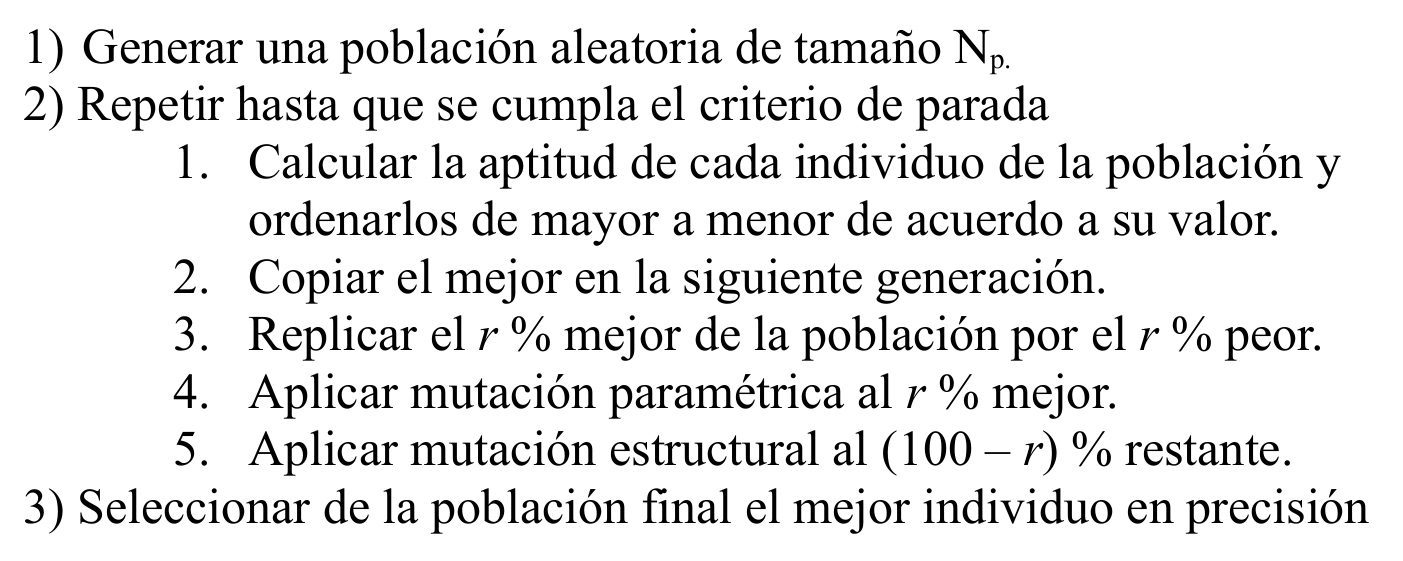
\includegraphics[keepaspectratio,width=11cm]{figuras/marcoNNEPMaeb2007.jpg}
% }
% \caption{Marco general de una variante del algoritmo CBFEP.}
% \label{CBFEPMaeb2007}
% \end{figure}
%
% Los resultados estadísticos (ver tabla IV en \cite{Hervas2007}) muestran que los modelos
% híbridos PSU no consiguen en media grandes diferencias con los modelos puros
% SU y PU, pero los mejores modelos obtenidos indican que las topologías
% híbridas son tan buenas como las mejores modelos puros, y además con un número de
% parámetros no significativamente superior (ver tabla V en \cite{Hervas2007}). En
%general,
% el número de nodos en capa oculta para un modelo híbrido es inferior o igual a los
% obtenidos por los puros (ver tabla III en \cite{Hervas2007}). Este trabajo deja abiertas
% varias cuestiones a tratar en un trabajo futuro:
% \begin{enumerate}
% 	\item A partir de las distribuciones de frecuencias asociadas a los patrones de los
% conjuntos de entrenamiento en problemas de clasificación y de las funciones de entropía
% cruzada, ¿es posible definir las características asociadas a la base de datos que
%determinen la familia de funciones (reconocedores universales) quees adecuada para
%mejorar la clasificación?
% 	\item ¿Podemos determinar algunas propiedades de las funciones de probabilidad a
% priori que permitan elegir entre diferentes familias de reconocedores universales, o
%bien
% entre la mezcla ''inteligente`` de diferentes modelos.
% 	\item ¿Es posible incorporar al algoritmo evolutivo procedimientos que permitan, en
% determinados momentos de la evolución, determinar el tipo de unidad que hay que incluir
%en
% el modelo para mejorar la precisión del clasificador en el conjunto de generalización?
% \end{enumerate}
%
% En \cite{Hervas2007a} se utiliza el mismo marco de trabajo o esquema de la figura
% \ref{CBFEPMaeb2007}, usando también modelos puros y modelos híbridos PSU. Para
% comprobar la precisión de los modelos obtenidos se usan una serie de bases de datos
% sintéticas gausianos multiclase con diferentes correlaciones lineales entre las
%variables
% de entrada y diferentes varianzas (ver sección 4 en \cite{Hervas2007a}). El método se
% compara con el análisis discriminante lineal (\textit{Linear Discriminant Analisys},
%LDA)
% \cite{Duda2000} y se ratifica
% que los modelos PSU obtienen, en la mayoría de los casos, iguales o mejores
% resultados que los modelos puros y que los obtenidos con LDA, no pudiendo éste
% último construir las funciones discriminantes en uno de los problemas, mientras que el
% modelo PSU obtiene una precisión del 100\% en generalización.
\paginavaciacompleta